%!TEX root = ../../common/main.tex

\chapter{The \acs*{LHCb} experiment}
\label{ch:lhcb_experiment}

The \ac{LHCb} collaboration operates a particle detector at the \ac{LHC}
located at \ac{CERN} in the Geneva area. The \LHCb experiment aims to study heavy
flavour physics by exploiting direct and indirect experimental techniques to its
full extent. Its physics program includes \CP violation measurements in $\B$ and
$\D$ meson decays
\cite{Aaij:2015tza,Aaij:2015yda,Aaij:2014uva,Aaij:2014fba,Aaij:2014dka,Aaij:2014zsa,Aaij:2014kxa}, 
the search for (very) rare decays \cite{CMS:2014xfa}, tests of
lepton-universality \cite{Aaij:2014ora,Aaij:2015yra}, as well as heavy flavour
spectroscopy \cite{Aaij:2014yka,Aaij:2015tga}.

In the next sections the experimental conditions at the \LHC and the design
of the \LHCb detector are outlined.

%%%%%%%%%%%%%%%%%%%%%%%%%%%%%%%%%%%%%%%%%%%%%%%%%%%%%%%%%%%%%%%%%%%%%%%%%%%%%%%%
\section{The \acs*{LHC} and its experiments}
\label{sec:lhcb_experiment:lhc}

With a circumference of \SI{26.7}{\kilo\metre} the \LHC is the largest man-made
particle accelerator. Using a \enquote{two-in-one} super-conducting magnet
design, two counter-rotating beams of protons (or ions) are intersected and
brought to collision at four interaction points, home of the large \LHC
experiments \acs*{ALICE}, \acs*{ATLAS}, \acs*{CMS}, and \acs*{LHCb}. The
collider's centre-of-mass energy of $\sqrt{s}=\SI{14}{\TeV}$ and a peak
luminosity of $L=\SI{e34}{\lumi}$ provide \LHC's experiments with high event
rates that are necessary in their searches for physics beyond the \SM.

Following approval in 1994, the \LHC re-used the existing \LEP tunnel and most
of its infrastructure after \LEP shut down in 2000. The \LHC---and former
\LEP---tunnel is built up of eight straight and eight arc sections and has a
internal diameter of $\SI{3.7}{\metre}$. It is located north-west of Geneva,
Switzerland at a depth between $\SI{45}{\metre}$ and $\SI{170}{\metre}$ below
the surface. The storage ring consists of superconducting NbTi magnets kept at
an operating temperature of $\SI{1.9}{\kelvin}$ by superfluid helium. A
superconducting \RF cavity system captures, accelerates, and stores the two
proton beams.

At design luminosity, $\num{2808}$ bunches with a bunch spacing of
$\SI{25}{\nano\second}$ are stored in each proton beam. The \LHC relies on a
supply chain of smaller accelerators providing the initial proton bunches.
\Cref{fig:lhcb_experiment:lhc:cern_accelerator_complex} depicts the \acs{CERN}
accelerator complex. A bottle of hydrogen gas is the source of the protons, that
are then subsequently accelerated to higher energies by the \LINACTwo, the
\BOOSTER, the \PSyn, and the \SPS, before being injected into the \LHC at an
energy of $\SI{450}{\GeV}$. The transfer lines Tl2 and Tl8 are used to inject
the proton bunches in both beam directions. As soon as the nominal number of
proton bunches is reached, the beam energies are increased up to $\SI{7}{\TeV}$
for each beam. The average \LHC turnaround time, \ie the time it takes to run
through the whole accelerator chain until a stable beam is achieved, adds up to
seven hours. Mainly due to beam loss from \pp collisions the beam intensities
and the instantaneous luminosity decay. Starting from a peak luminosity of
$L=\SI{e34}{\lumi}$ a luminosity lifetime of 15 hours is estimated. To prevent
uncontrolled beam losses and to protect the \LHC infrastructure and the \LHC
experiments a beam dump system is installed. The fully automated system monitors
the beam condition and is able to extract the beam from the \LHC using kicker
magnets in case of a failure. The beam dump system is also used regularly to
extract the beam after a successful run. For more information on the \LHC and
resident experiments, see \eg \Ref~\cite{Evans:2008zzb}.

\begin{figure}[t]
  %% trim={<left> <lower> <right> <upper>}
  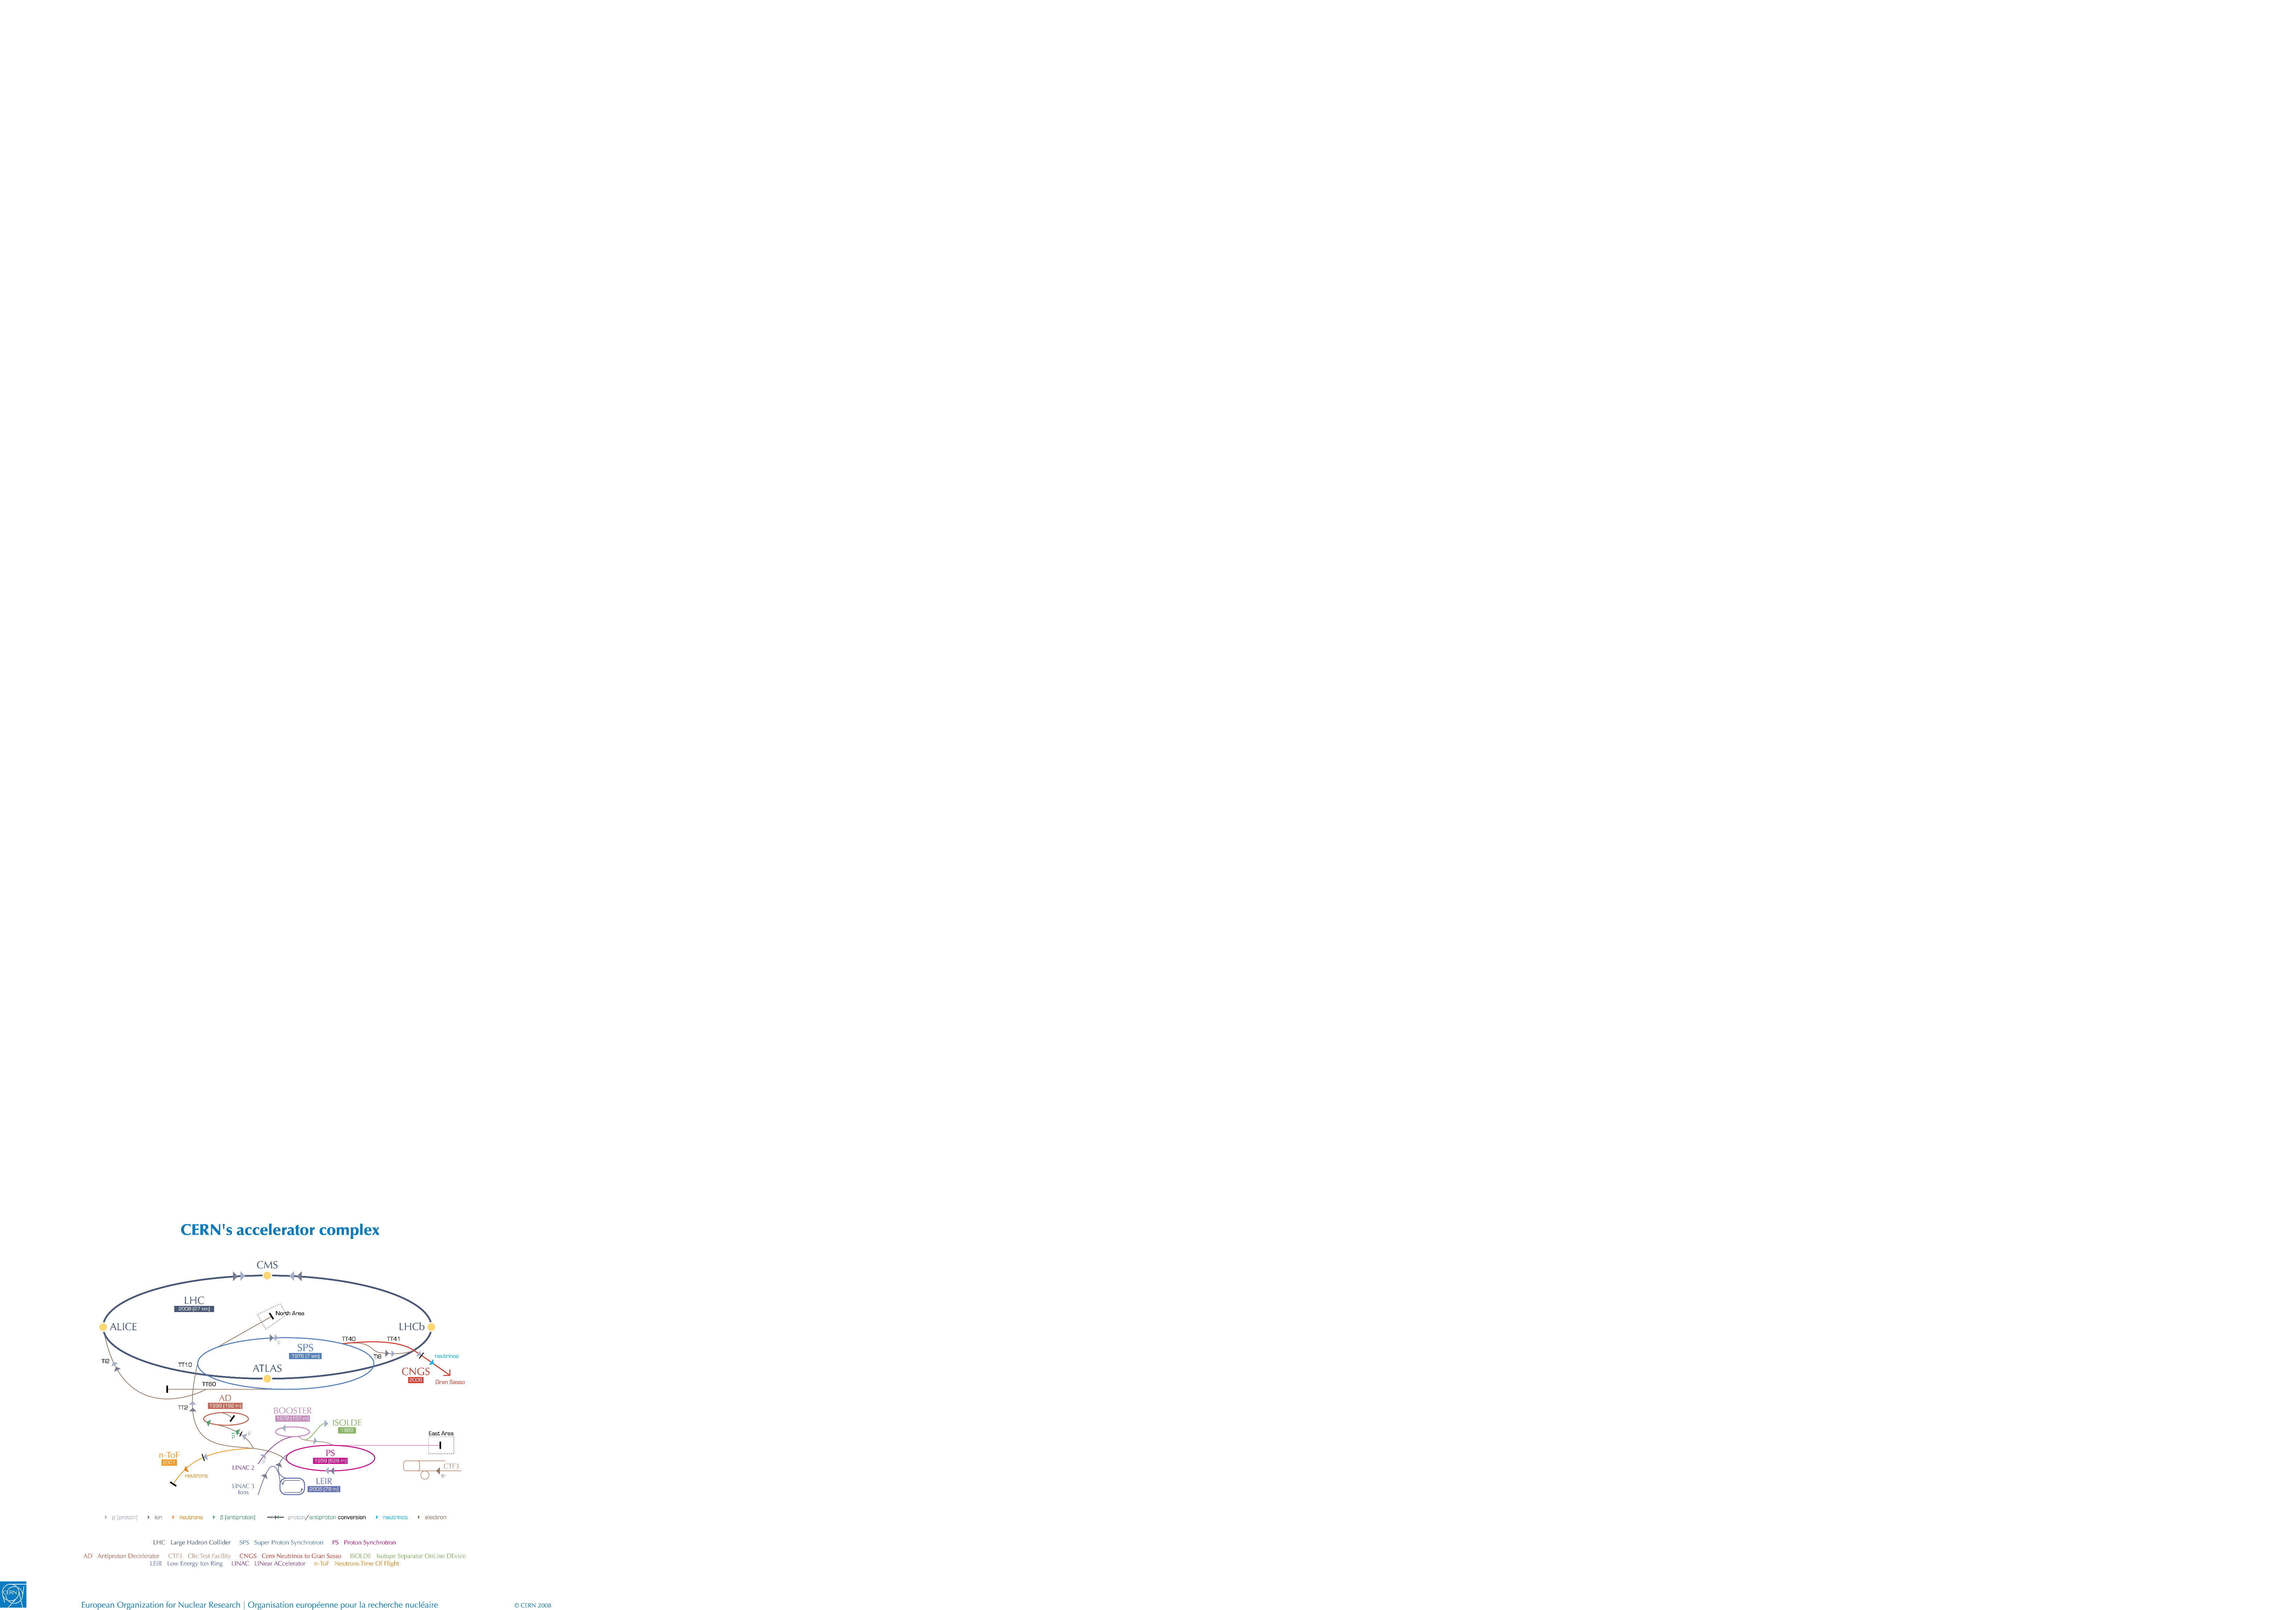
\includegraphics[width=\textwidth, trim={4.8cm 5.3cm 4.2cm 1.8cm}, clip=true]{private/content/the-lhcb-experiment/figs/cern_acceleator_complex.pdf}
  \caption{
  The \acs{CERN} accelerator complex \cite{Christiane:1260465}. Starting from
  the \acs{LINACTwo}, protons are accelerated through the \acs{BOOSTER}, the
  \acs{PSyn} and finally the \acs{SPS} before being injected into the \LHC. If
  one or both beams consist of heavy ions, the \acs*{LINACThree} and the
  \acs*{LEIR} are used to accelerate the ions and inject them into the
  \acs{PSyn}. }
  \label{fig:lhcb_experiment:lhc:cern_accelerator_complex}
\end{figure}

Shortly after the first successful circulation of two proton beams in September
2008, a fault occurred in the electrical bus connection between two magnets,
leading to a large helium leak and serious damage to several of \LHC's magnets
and infrastructure. After the incident, the management decided to reduce the
beam energy and intensity. Thus, in the years 2010 and 2011 the \LHC
centre-of-mass energy was $\sqrt{s}=\SI{7}{\TeV}$ with a bunch spacing of
$\SI{50}{\nano\second}$ delivering a peak instantaneous luminosity of
$\SI{2.4e33}{\lumi}$. An increase of the beam energy to $\sqrt{s}=\SI{8}{\TeV}$
lead to a peak instantaneous luminosity of $\SI{7.7e33}{\lumi}$ in 2012
\cite{Lamont:2013cma}.

The \LHC is not only capable of colliding protons but also lead ions in Pb-Pb as
well as in \proton-Pb and Pb-\proton collisions. For this purpose the
\acs{ALICE} (\acl{ALICE}) detector \cite{Aamodt:2008zz} is specifically designed
to study QCD interactions and the quark-gluon plasma produced in the \LHC ion
runs, where it has to cope with very large particle multiplicities. In the case
of an heavy ion run, the
\LINACThree and the \LEIR mark the starting point of the accelerator chain,
before injecting the lead ions into the \PSyn.

In total, seven experiments are located at the four interaction regions of the
\LHC. The two multi-purpose detectors \acs{ATLAS} (\acl{ATLAS})
\cite{Aad:2008zzm} and \acs{CMS} (\acl{CMS}) \cite{Chatrchyan:2008aa} are
installed at opposite sides of the storage ring. Both experiments cover a great
variety of physics activities: the search for scalar particles, particles
predicted by super-symmetric models, dark matter candidates, and evidence for
extra spacial dimensions. Around the interaction regions of the \CMS experiment,
the \acs{TOTEM} (\acl{TOTEM}) detectors \cite{Anelli:2008zza} are located.
Together with the \LHCf experiment \cite{Adriani:2008zz}, located on both sides
of the \ATLAS interaction region, the detectors are designated to address the
study of the \enquote{forward} region of the collisions at very small angles to
the beam direction. The seventh experiment \acs{MoEDAL} (\acl{MoEDAL}) extends
the \LHC physics program to the direct search for magnetic monopoles. Still
missing in this list, is the \LHCb experiment, that will be explained in more
detail in the next section.

% to enforce definition of abbreviations
\acuse{LINACThree,LEIR,ALICE,ATLAS,CMS,TOTEM,MoEDAL,LHCf}

%%%%%%%%%%%%%%%%%%%%%%%%%%%%%%%%%%%%%%%%%%%%%%%%%%%%%%%%%%%%%%%%%%%%%%%%%%%%%%%%
\section{The LHCb detector}
\label{sec:lhcb_experiment:detector}

The \LHCb detector is a unique precision instrument solely designed to study \CP
violation and rare decays of beauty and charm hadrons
(\cref{fig:lhcb_experiment:detector:overview}). It is constructed as a
single-arm spectrometer covering an angular range from approximately
$\SI{10}{\mrad}$ to $\SI{300}{\mrad}$ ($\SI{250}{\mrad}$) in the horizontal
(vertical) plane.
%
\begin{figure}[t]
  \centering
    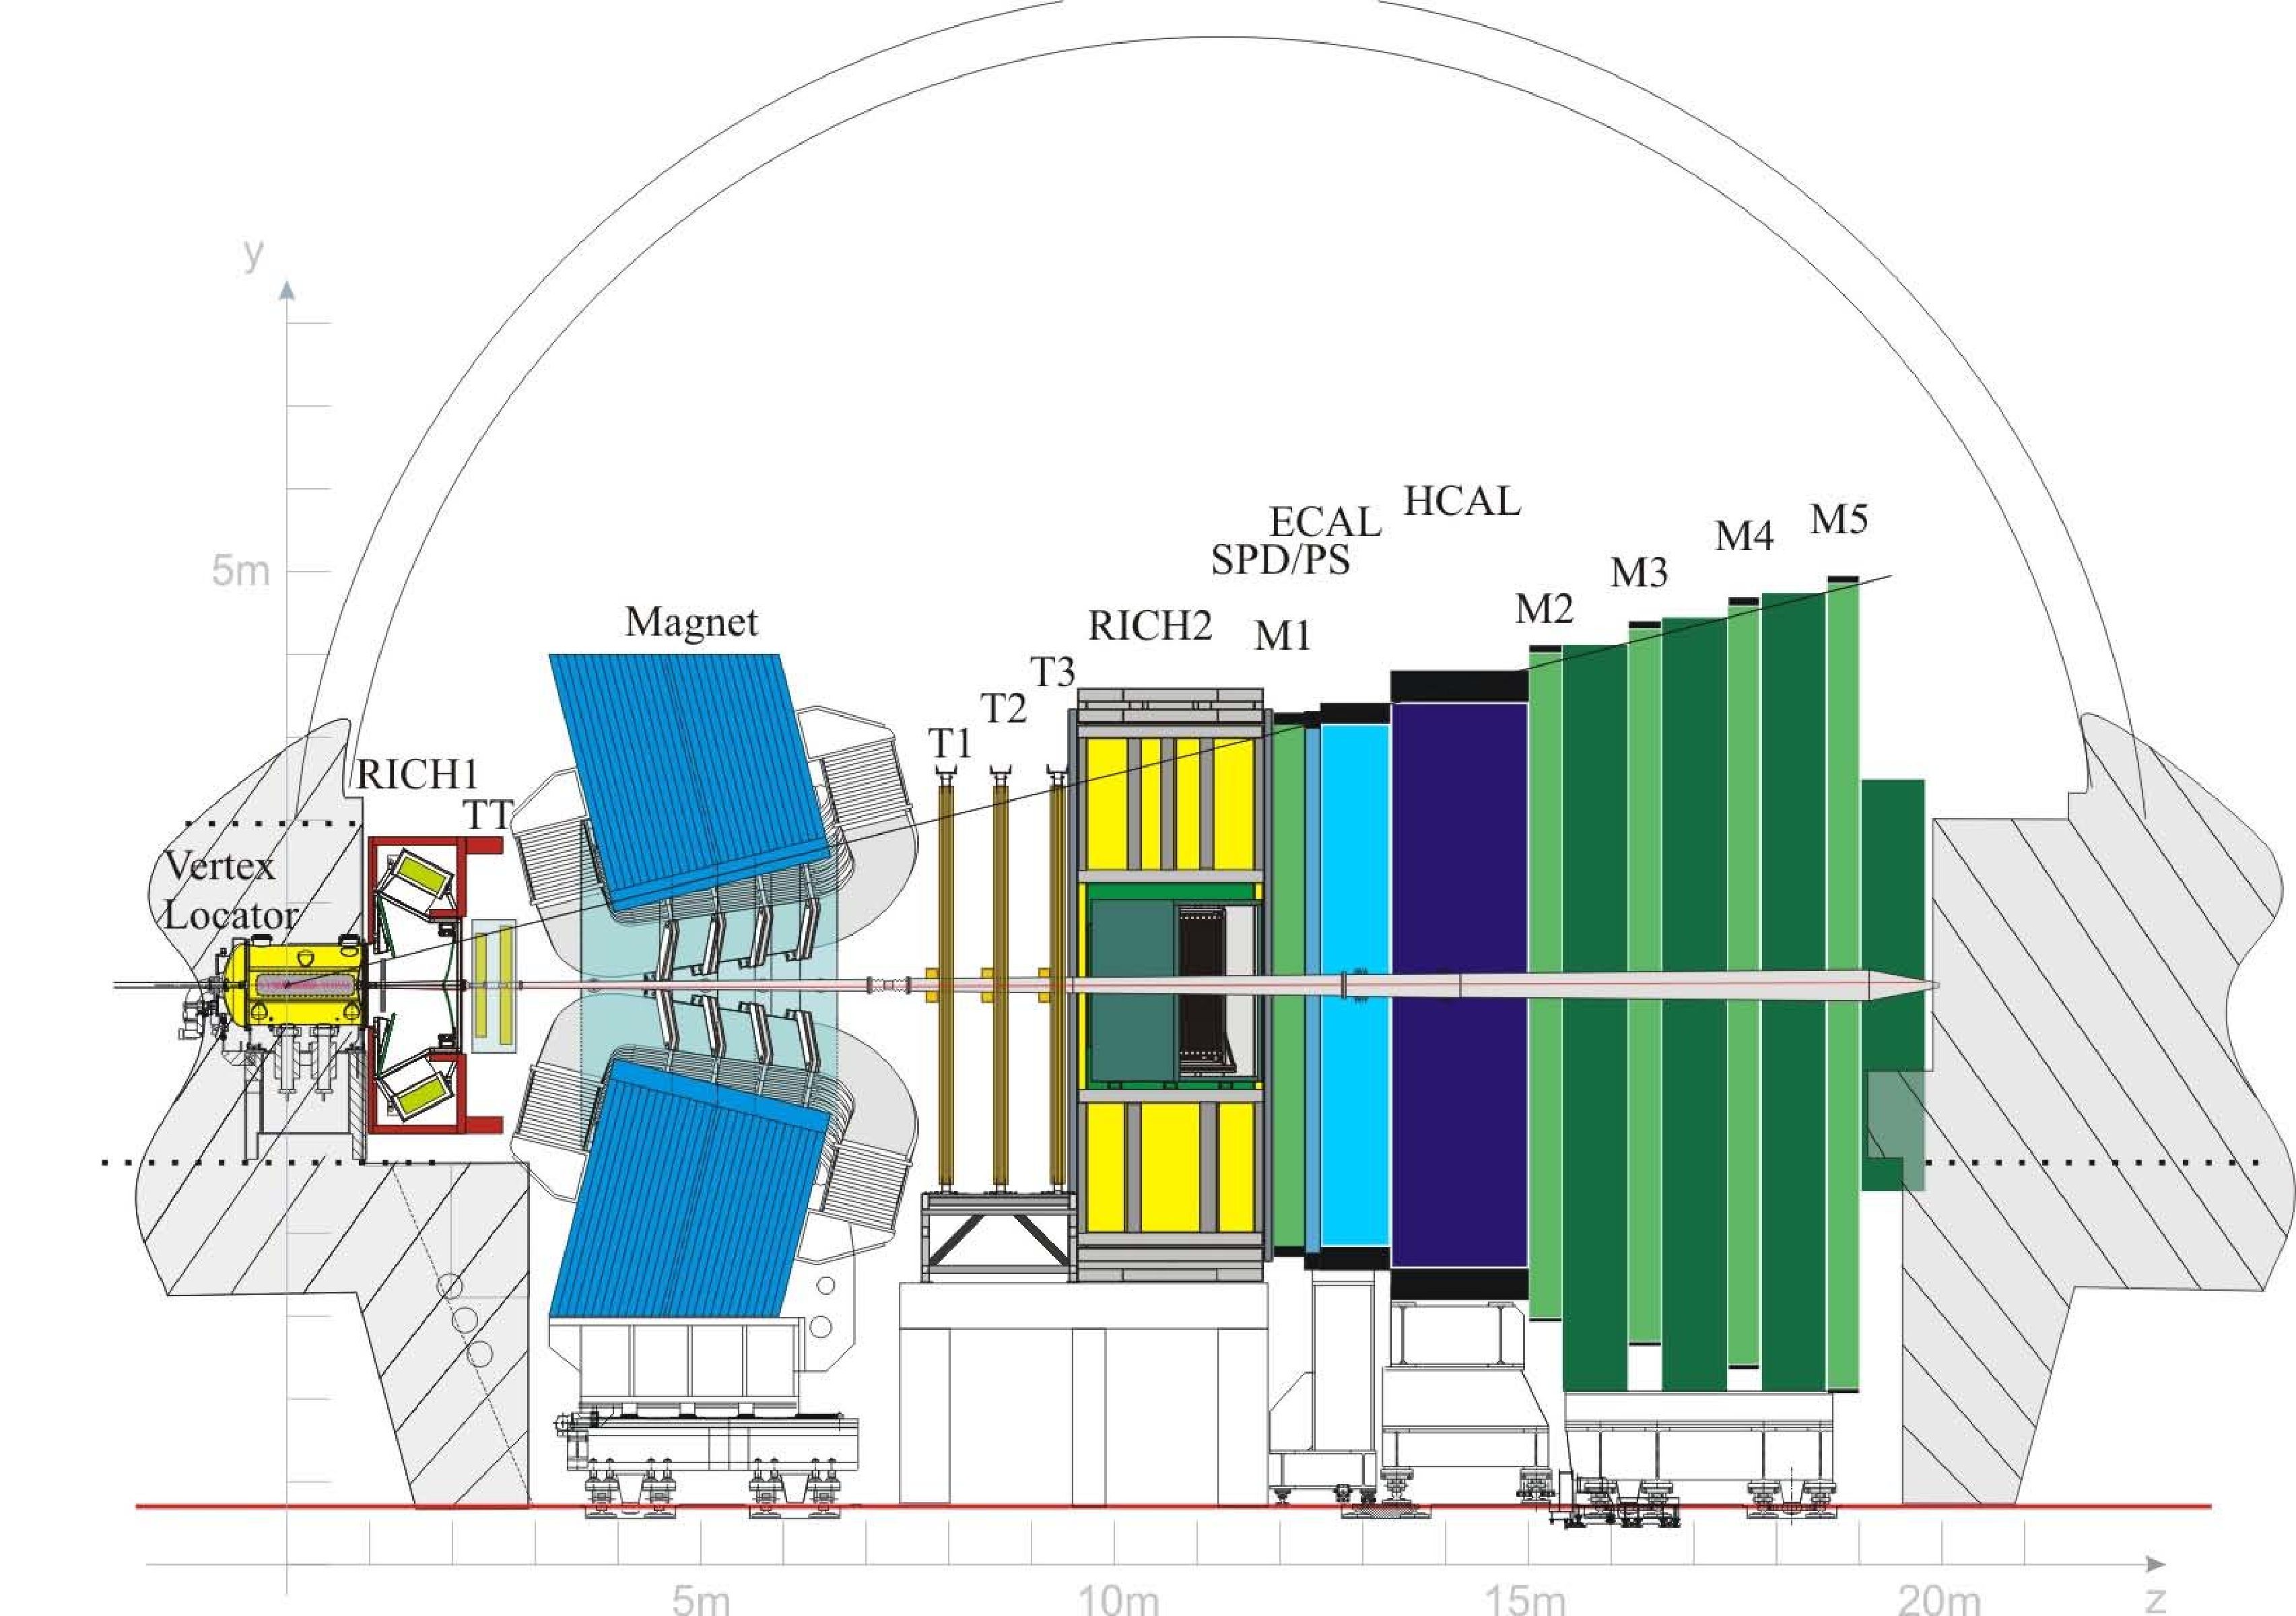
\includegraphics[width=\textwidth]{private/content/the-lhcb-experiment/figs/lhcb_detector_overview.pdf}
  \caption{
    Schematic cross section of the \acs{LHCb} detector in the $(y,z)$ plane at
  $x=0$. The \protonproton interaction region is located at the coordinates
  $(0,0,0)$ on the left side of the figure. The beam pipe crosses the detector at
  $(0,0,z)$. The main interaction region is surrounded by the \acs*{VELO},
  following the \acs*{RICH}1 and the \acs*{TT}. On the right side of the magnet
  the three tracking stations (T1-3) consisting of the \acs*{IT} and the
  \acs*{OT} are installed. Further on, the \acs*{RICH}2, the calorimeter system
  (\acs*{SPD}, \acs*{PS}, \acs*{ECAL}, and \acs*{HCAL}), and the muon system
  (M1-5) is located. }
  \label{fig:lhcb_experiment:detector:overview}
\end{figure}
%
The detector layout exploits the characteristics of the heavy flavour production
in \protonproton collisions at the \LHC. The production of heavy quarks in an
hadronic environment is dominated by quark pair production in gluon-gluon fusion
$\gluon\gluon\to\bbbar/\ccbar$ and quark-antiquark annihilation
$\qqbar\to\bbbar/\ccbar$.

The heavy quark production cross-sections depend on the centre-of-mass energy
$\sqrt{s}$ of the \protonproton collision. As illustrated in
\cref{fig:lhcb_experiment:detector:cross_section} the $\bbbar$ pair
cross-section behaves approximately linearly with $\sqrt{s}$ and lies roughly in
the order of $\SI{300}{\microbarn}$ for $\sqrt{s}=\SI{7}{\TeV}$.
%
\begin{figure}[t]
  \centering
    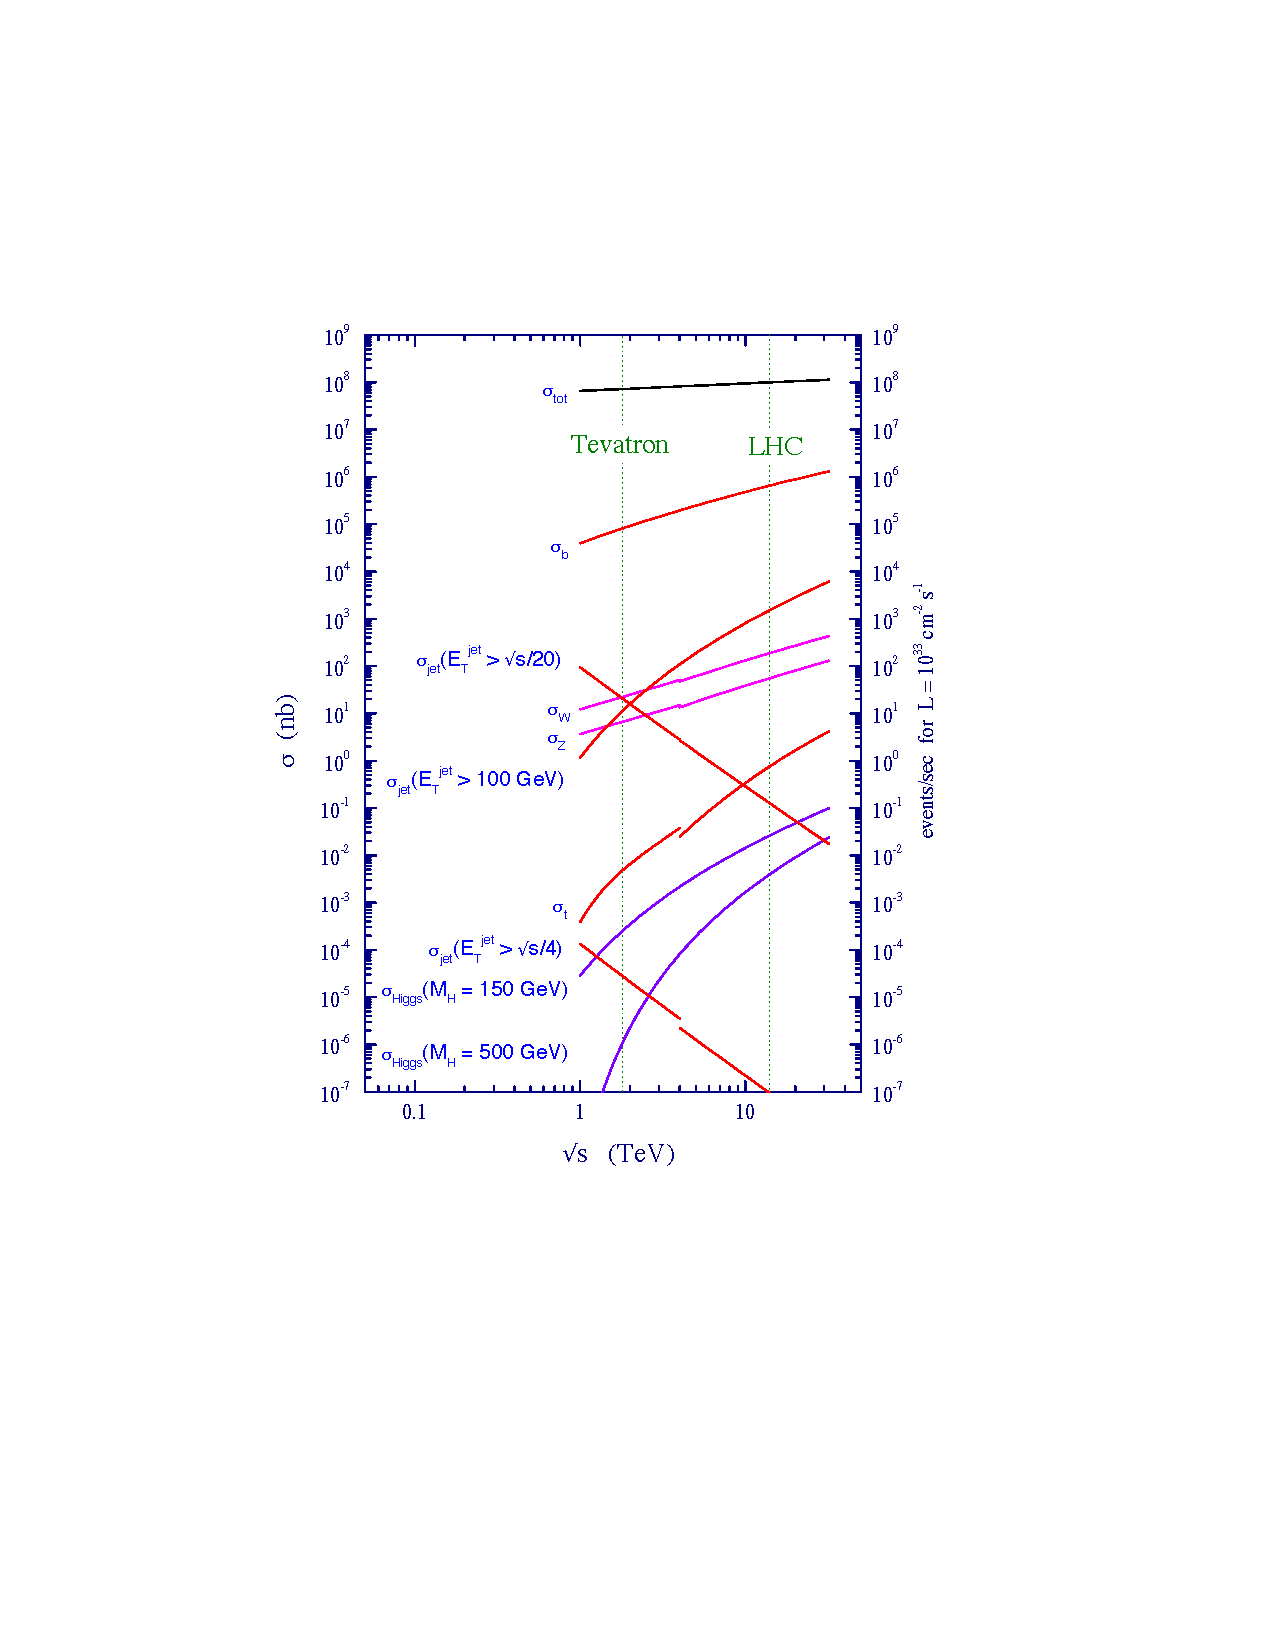
\includegraphics[width=0.6\textwidth]{private/content/the-lhcb-experiment/figs/lhc_cross_sections.pdf}
  \caption{
    Production cross-sections as a function of the \acl{protonproton} collision centre-of-mass energy. \cite{Campbell:2006wx}
  }
  \label{fig:lhcb_experiment:detector:cross_section}
\end{figure}
%
At \LHC energies the partons involved in the collisions are likely to carry very
different momenta, leading to a strong boost of the produced quark pair in
direction of the beam axis. Thus, the produced quarks have a high probability of
being produced at a small azimuthal angle $\theta_{1,2}$ with respect to the
beam axis. \Cref{fig:lhcb_experiment:detector:production} illustrates the the
correlation of the two quark angles $\theta_{1}$ and $\theta_{2}$. The red
shaded region marks the \LHCb detector acceptance where around
$\SI{25}{\percent}$ of all produced $\bbbar$ quark pairs are found.

The acceptance is depicted as well in
\cref{fig:lhcb_experiment:detector:production} as a function of the quark
\acl{pseudorapidity} $\text{\acs{pseudorapidity}} = -\ln(\tan(\theta/2))$. Here
the \LHCb acceptance region ($\num{1.8} < \eta < \num{4.9}$) can be identified
by the red rectangle while the acceptance of the \acfp{GPD} \ATLAS and \CMS is
marked by the yellow rectangle.
%
\begin{figure}[t]
  \centering
    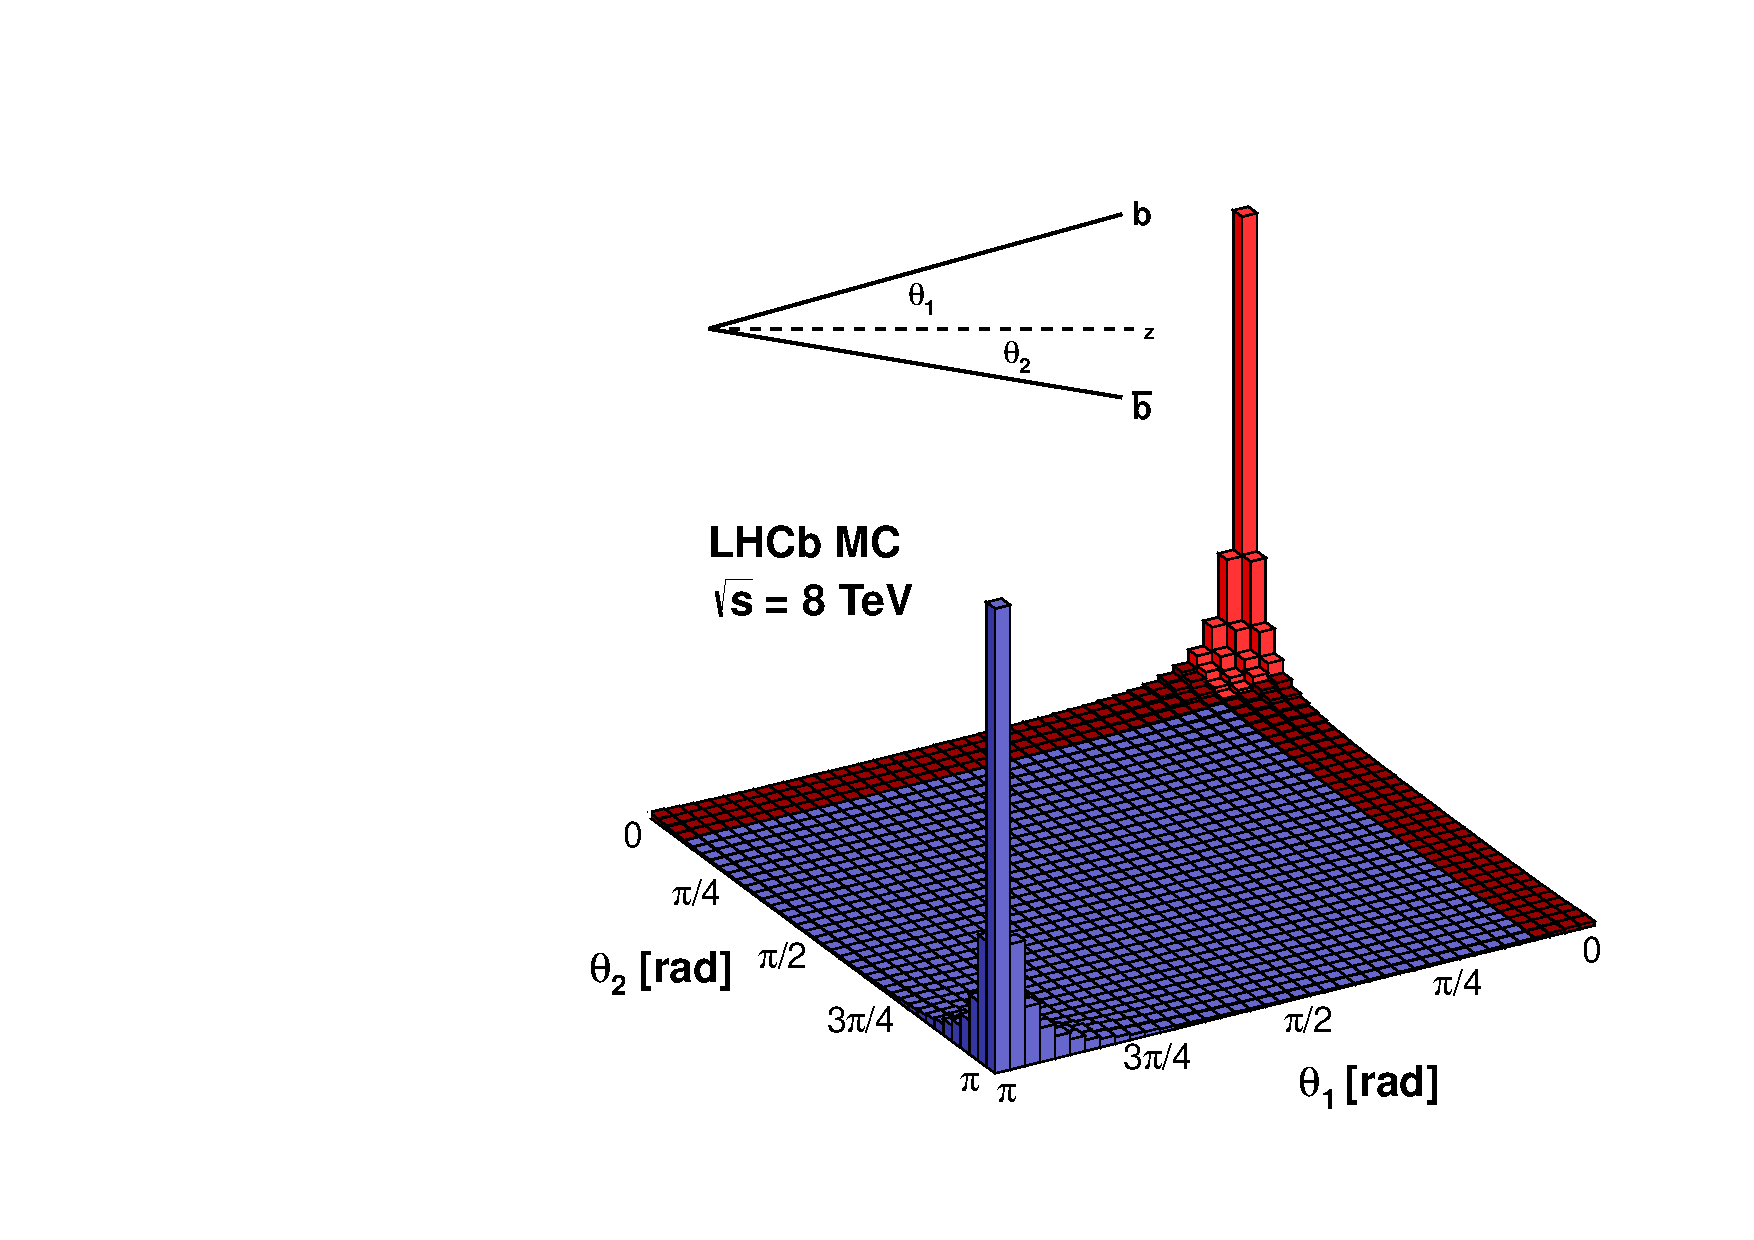
\includegraphics[width=0.48\textwidth]{private/content/the-lhcb-experiment/figs/lhcb_quark_correlation.pdf}
    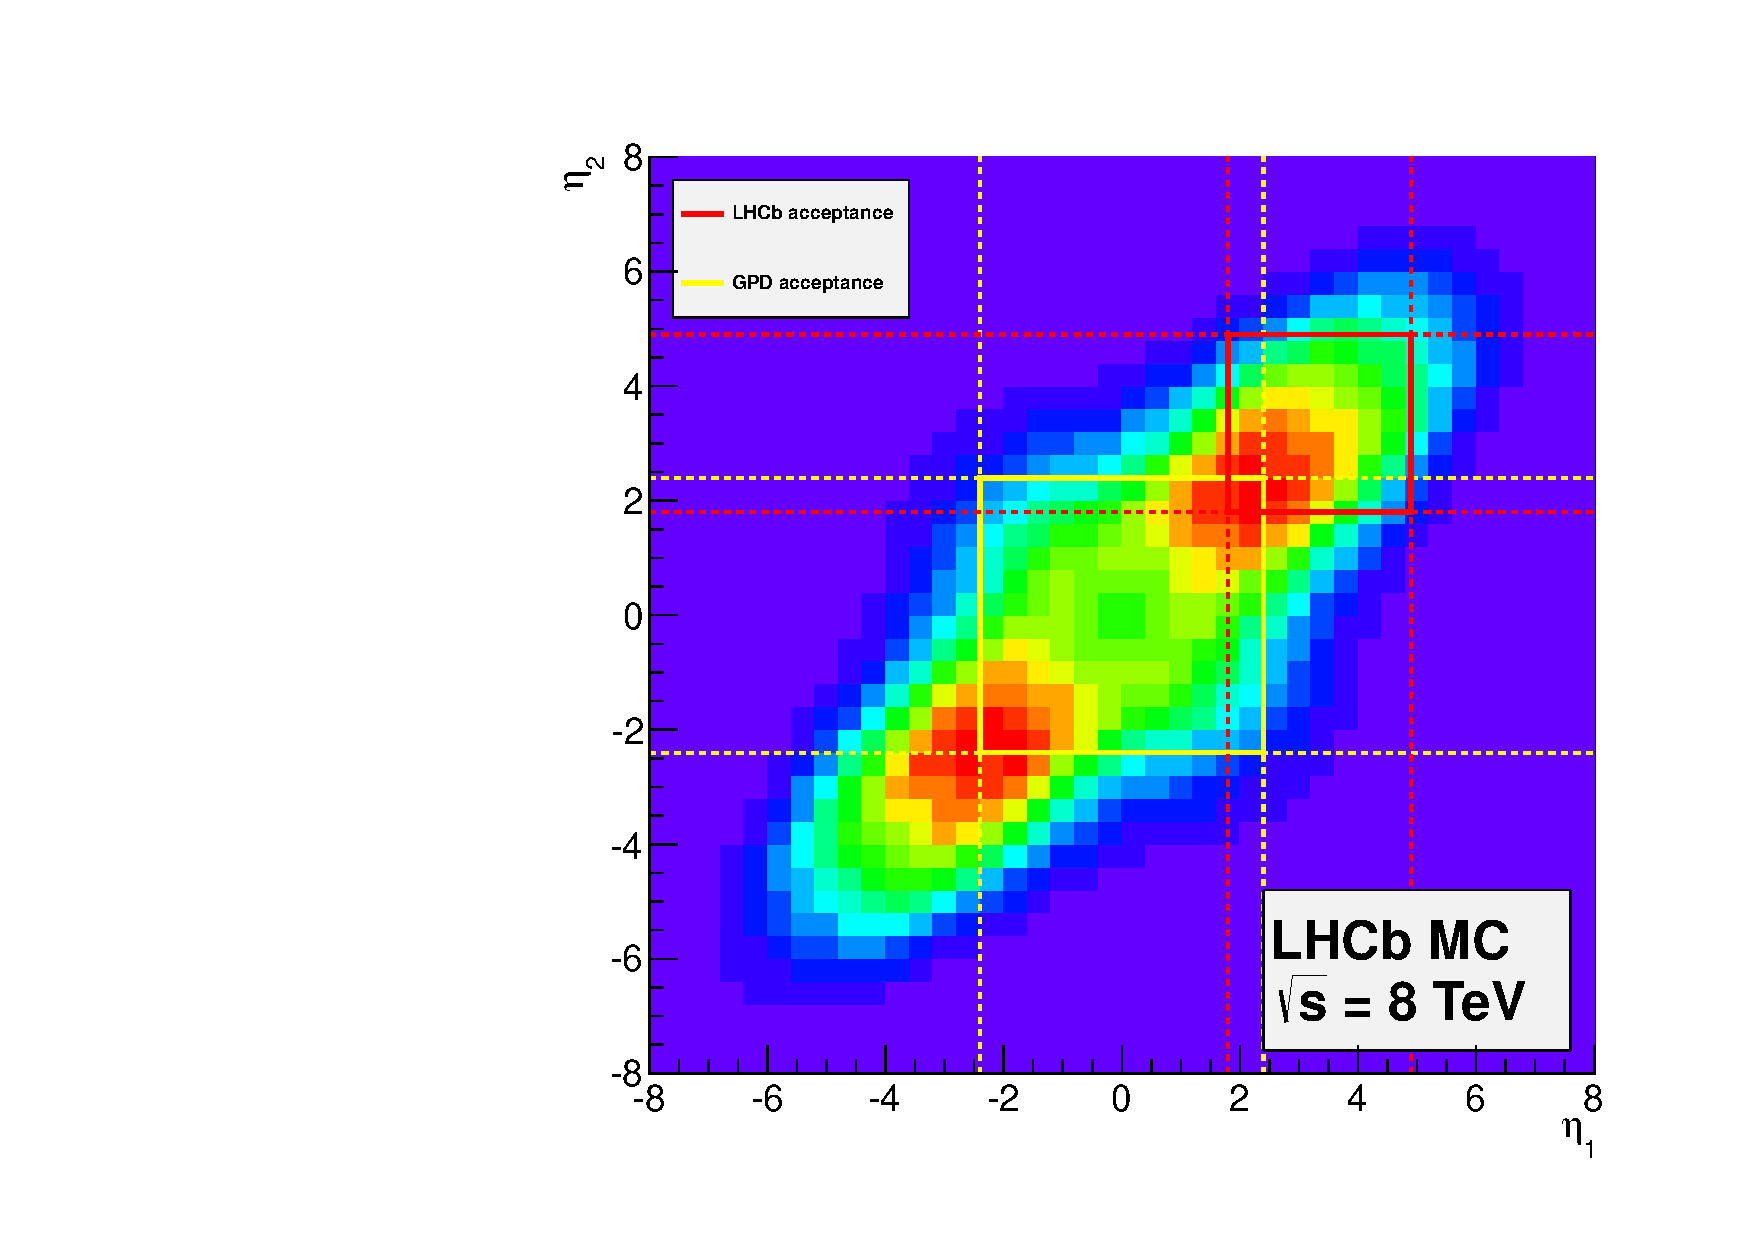
\includegraphics[width=0.48\textwidth]{private/content/the-lhcb-experiment/figs/lhcb_acceptance.pdf}
  \caption{
    Plots of the $\bbbar$ quark pair production numbers (in arbitrary units) at
  a centre-of-mass energy of $\sqrt{s} = \SI{8}{\TeV}$ as a function of (left)
  the azimuthal angles $\theta_{1,2}$ and (right) the \acf{pseudorapidity}.
  (Left) The red shaded region or (right) the red rectangle mark the \LHCb
  detector acceptance. \cite{lhcb:quarkproduction}}
  \label{fig:lhcb_experiment:detector:production}
\end{figure}
%

After production each $\bquark$ quark hadronises independently forming a
\bhadron. Most likely by bounding to a light quark forming a $\Bu$ or a $\Bd$
(\SI{40}{\percent} each), to heavier quarks as in $\Bs$ (\SI{11}{\percent}) or
even $\bquark$ baryons as $\Lambdab$ (\SI{9}{\percent}). The numbers in
parenthesis denote the fraction of the total production in percent
\cite{Agashe:2014kda}. 

At this point, flavour conjugate states are implied as the production is in
principle symmetric in quark flavour. However, as the
\protonproton collision defines an initial state with positive charge and in
absence of any valence anti-quarks, different production rates are expected
\cite{Chaichian:1993rh,Norrbin:2000zc,Norrbin:2000jy}. As this influences the
flavour-sensitive \CP violation measurement, precautions are taken as described
in \cref{sec:measurement_of_sin2beta:likelihood_fit:model:decay_time}.

%%%%%%%%%%%%%%%%%%%%%%%%%%%%%%%%%%%%%%%%%%%%%%%%%%%%%%%%%%%%%%%%%%%%%%%%%%%%%%%%
\section{Track reconstruction}
\label{sec:lhcb_experiment:tracking}

The \LHCb track reconstruction is based on information from a set of tracking
detectors located around a spectrometer magnet with an integrated field of
$\SI{4}{\tesla\metre}$. The tracking system consists of the \VELO, the \TT, the
\IT and the \OT. Silicon microstrips are used in the first three, while the
latter is constructed as a drift-time detector. The \VELO is described in
\cref{sec:lhcb_experiment:tracking:velo}, the \TT and the \IT in
\cref{sec:lhcb_experiment:tracking:ttit}, and the \OT in
\cref{sec:lhcb_experiment:tracking:ot}.

%%------------------------------------------------------------------------------
\subsection{The \acl*{VELO}}
\label{sec:lhcb_experiment:tracking:velo}

Surrounding the \protonproton interaction region the \VELO's main purpose is the
precise position measurement of traversing particles to reconstruct the \ac{PV}
and displaced \acp{SV}. To achieve the best possible spatial resolution the
sensors must be positioned close to the beam trajectory. To allow the sensors to
be as close as $\SI{8}{\milli\metre}$ to the interaction region and still
prevent damage during beam injection, the \VELO modules are split in two halves
and can be retracted until stable beams are present. Each single module consists
of two half-disk shaped silicon microstrip sensor modules covering either the
radial dimensions ($R$ sensor) or the angular dimension ($\Phi$ sensor) as can
be seen in the schematic visualisation in
\cref{fig:lhcb_experiment:tracking:velo:sensor}.
%
\begin{figure}[t]
  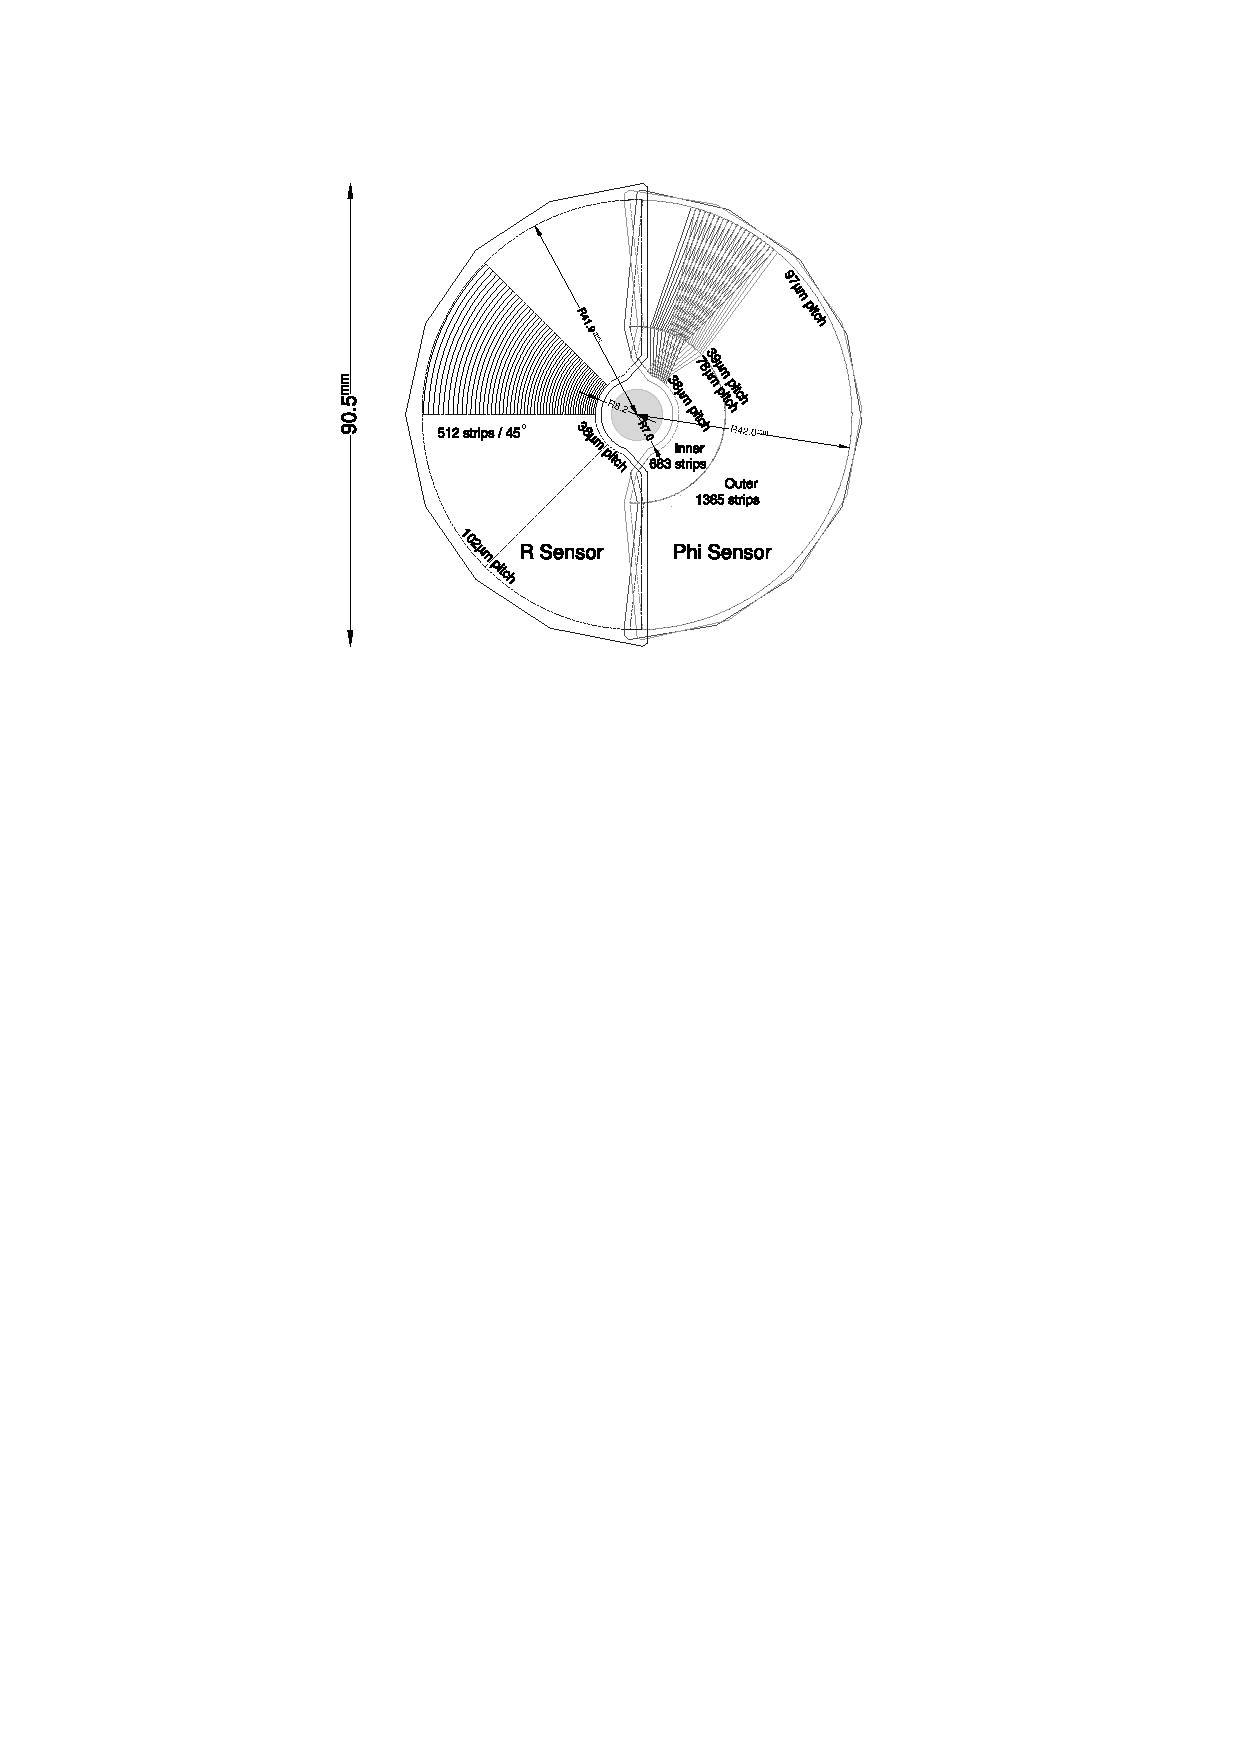
\includegraphics[width=0.42\textwidth]{private/content/the-lhcb-experiment/figs/lhcb_detector_velo_sensors.pdf}
  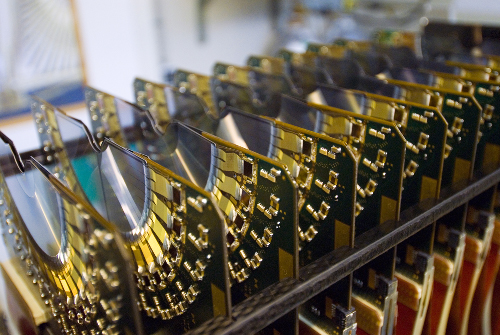
\includegraphics[width=0.55\textwidth]{private/content/the-lhcb-experiment/figs/lhcb_detector_velo_assembly.jpg}
  \caption{(Left) Schematic representation of the $R$ and $\Phi$ sensor for one
  of the \VELO modules \cite{Alves:2008zz}. (Right) Picture of the \VELO during
  assembly \cite{Aaij:1707015}. }
  \label{fig:lhcb_experiment:tracking:velo:sensor}
\end{figure}
%
The \VELO covers the total \LHCb acceptance region, such that all tracks cross
at least three \VELO stations. \Cref{fig:lhcb_experiment:tracking:velo:overview}
shows the cross section of the \VELO in the $(x,z)$ plane at $y=0$ with all
modules visible.
%
\begin{figure}[t]
  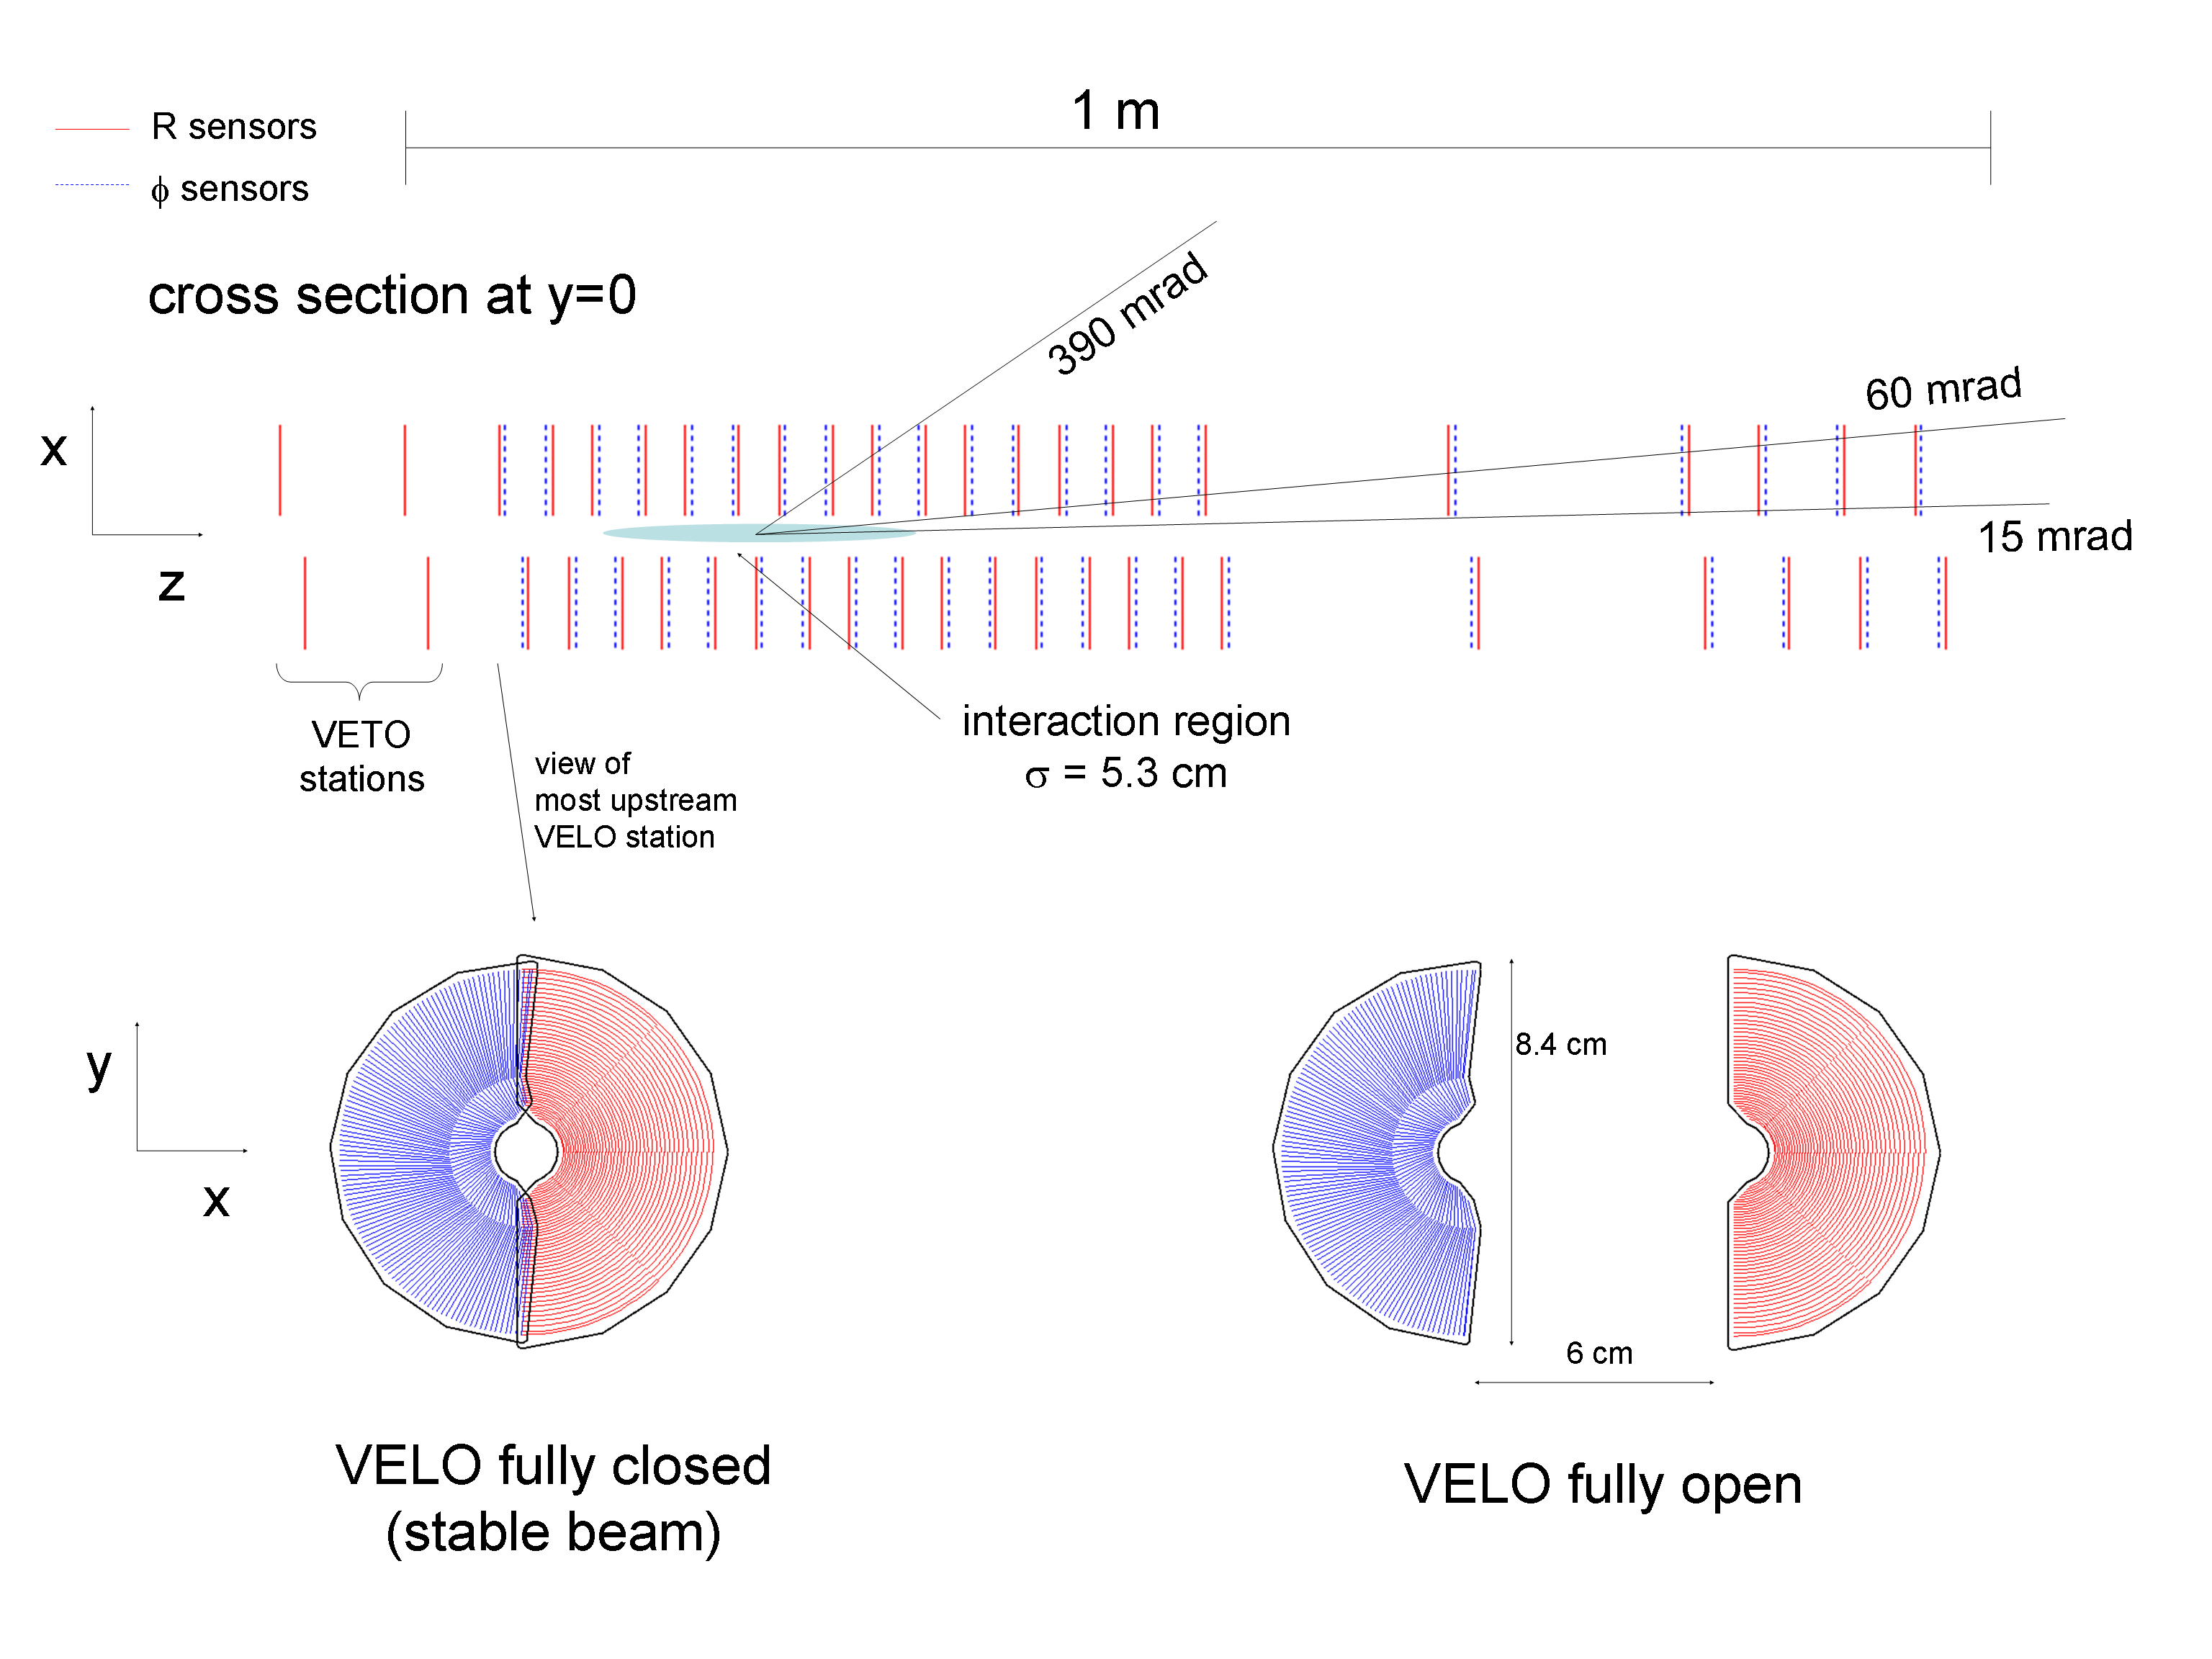
\includegraphics[width=\textwidth]{private/content/the-lhcb-experiment/figs/lhcb_detector_velo_overview.png}
  \caption{
    Cross section of the closed \VELO in the $(x,z)$ plane at $y=0$ \cite{Alves:2008zz}.
  }
  \label{fig:lhcb_experiment:tracking:velo:overview}
\end{figure}

% \begin{itemize}
%   \item purpose: displaced secondary vertices, decay length, decay time, IP
%   \item silicon modules in r and phi, geometrical dimensions, mechanical accuracy, closest approach to beam
%   \item acceptance: 1.6 < eta < 4.9; |z| < 10.6cm
%   \item requirement of at least three hits in the VELO stations
%   \item pile-up veto system
%   \item retractable, RF foil, in vacuum (primary and secondary)
%   \item hardware interlock system
%   \item performance(?)
% \end{itemize}
%%------------------------------------------------------------------------------
\subsection{The \acs*{LHCb} tracking system}
\label{sec:lhcb_experiment:tracking:ttit}
\label{sec:lhcb_experiment:tracking:ot}

The \TT as well as the \IT make use of silicon microstrip sensors to track
particle trajectories. The planar \TT station is located upstream of the magnet
and is $\SI{150}{\centi\metre}$ wide and $\SI{130}{\centi\metre}$ high. The
three \IT stations are on the downstream side of the magnet and cover a central
region around the beam pipe that is $\SI{120}{\centi\metre}$ wide and
$\SI{40}{\centi\metre}$ high. Each of the stations has four detector layers,
where the strips in the two inner layer are rotated $\pm\SI{5}{\degree}$ to
allow for two dimensional positioning.

The outer region of the three downstream tracking stations, called \OT, consists
of a drift-time detector constructed from an array of gas-filled straw-tube
modules. The large planar detector spans an active area of $\SI[product-units =
power]{6 x 5}{\metre}$. With drift times smaller than $\SI{50}{\nano\second}$
and a drift-coordinate resolution of $\SI{20}{\micro\metre}$ the \OT allows for
tracking in the low occupancy region around the \IT.

%%------------------------------------------------------------------------------
\subsection{Track reconstruction technique and performance}
\label{sec:lhcb_experiment:tracking:techniques_and_performance}

The reconstruction of trajectories employs all available tracking information
from \VELO, \TT, \IT, and \OT \cite{Aaij:2014pwa}. Each track is classified by
the position of associated hits in the different subsystems
(\cref{fig:lhcb_experiment:tracking:techniques_and_performance:tracktypes}).
\emph{T tracks} only have hits in the \IT and \OT, \emph{\VELO tracks} only have
hits in the
\VELO, \emph{upstream tracks} only have hits in the \VELO and \TT. Tracks
leaving hits in all tracking systems are called \emph{long tracks}, while tracks
with hits in each system except the \VELO are called \emph{downstream tracks}.
%
\begin{figure}[t]
  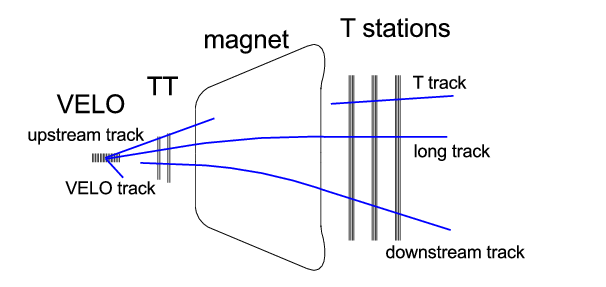
\includegraphics[width=\textwidth]{private/content/the-lhcb-experiment/figs/lhcb_track_types.png}
  \caption{
    Illustration of the \LHCb tracking subsystems and track type definitions \cite{Aaij:2014pwa}.
  }
  \label{fig:lhcb_experiment:tracking:techniques_and_performance:tracktypes}
\end{figure}
%
Starting from \VELO hits and with the knowledge of the magnetic field map,
tracks are reconstructed using extrapolations of the straight track sections
outside the magnet to the upstream tracking stations (\IT/\OT). If \TT hits are
present they are considered as well. The reconstruction of downstream tracks
starts from hits in in the upstream tracking stations that are then
extrapolation through the magnet and combined with hits in the \TT. Other track
types are reconstructed in similar ways. 

Obviously long tracks carry the most information and are preferred.
Nevertheless, other types of reconstructed tracks are useful too. \VELO tracks
are employed to improve the identification of \PV positions, T and upstream
tracks can be utilised to enhance the \RICH performance, and downstream tracks
increase the number of reconstructed \KS and other long lived particles that may
decay outside the \VELO acceptance.

The average reconstruction efficiency of tracks inside the detector acceptance
and in the momentum range between 
$\SIrange[range-phrase = -,range-units = single]{5}{200}{\GeV}$ is better than
$\SI{95}{\percent}$. The track uncertainty is below $\SI{0.5}{\percent}$ for
muons and below $\SI{1.5}{\percent}$ for pions and kaons. The high quality of
the tracking algorithms has a direct effect on the momentum resolution ($\Delta
p/p = \SIrange[range-phrase = -,range-units = single]{0.4}{0.6}{\percent}$), the
invariant mass resolution ($\SIrange[range-phrase = -,range-units =single]{12}{25}{\MeVcc}$ 
for $\BdToJpsiX$ decays), the impact parameter resolution (\sim$\SI{20}{\micro\metre}$), 
and finally provides an excellent decay time resolution of around
$\SI{45}{\ps}$ \cite{lhcb:performance}.

%%%%%%%%%%%%%%%%%%%%%%%%%%%%%%%%%%%%%%%%%%%%%%%%%%%%%%%%%%%%%%%%%%%%%%%%%%%%%%%%
\section{Particle identification}
\label{sec:lhcb_experiment:pid}

The \LHCb \PID system consists of two \acp{RICH}, up- and downstream of the
magnet, the calorimeter system, and the muon system. Based on the information
from the \PID systems a likelihood for a given particle hypothesis is
determined. The \acp{RICH} are further described in
\cref{sec:lhcb_experiment:pid:rich}, the calorimeter system in
\cref{sec:lhcb_experiment:pid:calo}, and the muon system in
\cref{sec:lhcb_experiment:pid:muon}.

%%------------------------------------------------------------------------------
\subsection{The \aclp*{RICH}}
\label{sec:lhcb_experiment:pid:rich}

Exploiting the radiation emitted by a charged particle moving through a medium
at a speed greater than the speed of light, the two \acp{RICH} are used to
distinguish between pions, kaons, and protons. As illustrated in
\cref{fig:lhcb_experiment:tracking:pid:radiator} the cherenkov angle
$\Theta_\mathrm{C}$ shows a strong momentum dependence and therefore different
radiators are used to get a particle hypothesis for low- and high-momentum
particles. The detectors make use of a system of flat and spherical mirrors to
reflect the emitted light to \acp{HPD}.

\RICH{}1 is located upstream of the magnet in between the \VELO and the \TT, it
contains aerogel and \fluorocarbonfour gas radiators, and provides \PID for
particles with low momenta from $\SIrange[range-phrase = \text{ to },range-units
= single]{1}{60}{\GeVc}$. \RICH{}2 is located after the last tracking station,
it uses \fluorocarbon gas as a radiator and allows \PID for particles in the
range from $\SIrange[range-phrase = \text{ to },range-units =
single]{15}{\geq100}{\GeVc}$.
%
\begin{figure}[t]
  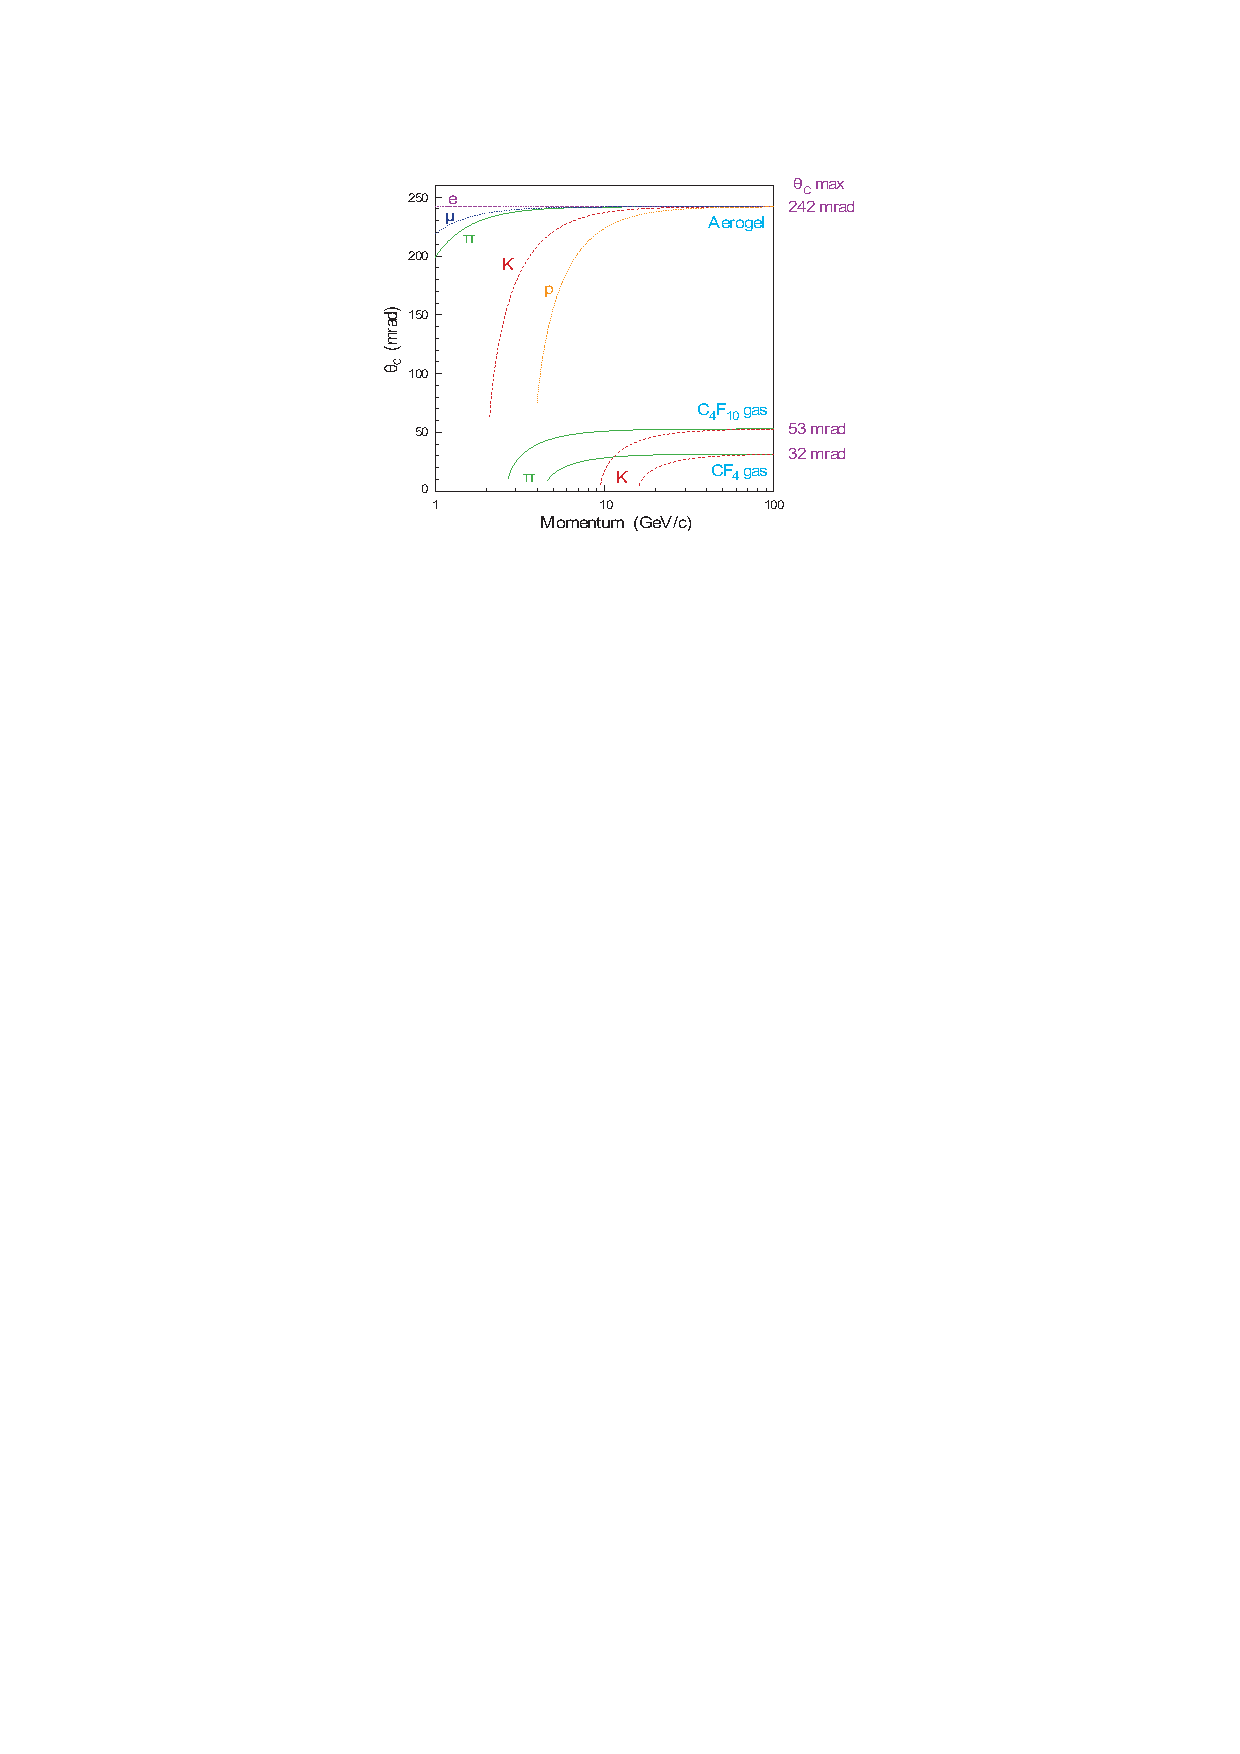
\includegraphics[width=0.48\textwidth]{private/content/the-lhcb-experiment/figs/lhcb_detector_rich_momentum.pdf}
  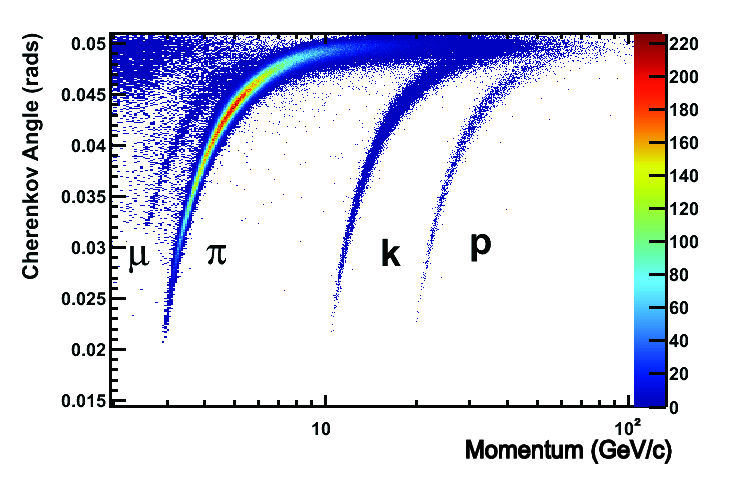
\includegraphics[width=0.48\textwidth]{private/content/the-lhcb-experiment/figs/lhcb_detector_rich_radiator.png}
  \caption{Momentum dependence of the cherenkov angle $\Theta_\mathrm{C}$ for
  (left) all \RICH radiators \cite{Alves:2008zz} and (right) for the
  \fluorocarbonfour radiator only \cite{Adinolfi:2012qfa}.}
  \label{fig:lhcb_experiment:tracking:pid:radiator}
\end{figure}

%%------------------------------------------------------------------------------
\subsection{The calorimeter system}
\label{sec:lhcb_experiment:pid:calo}

The \LHCb calorimeter system is used for both trigger
(\cref{sec:lhcb_experiment:trigger}) and \PID. It consists of an
\ECAL---including the \SPD and the \PS---followed by a \HCAL. All the
calorimeter sub-systems make use of the scintillation light originating from
traversing charged particles that is collected and transmitted by fibres to
\acp{PMT}.

First, the \SPD selects charged particles, secondly the \PS provides separation
of charged pions and electrons. Finally the \ECAL measures the energy deposition
and position of electromagnetic showers. The \HCAL is a massive
$\SI[product-units = power]{8.4 x 6.8}{\metre}$ planar, $\SI{500}{\tonne}$
detector, build-up from alternating iron plates and scintillating tiles,
providing energy measurements of hadronic showers.

%%------------------------------------------------------------------------------
\subsection{The muon system}
\label{sec:lhcb_experiment:pid:muon}

The muon system consists of five stations of \acp{MWPC}, provides muon \PID and
serves as a high \pT trigger. The system is located in front of (M1) and behind
(M2-M5) the calorimeter system. It is especially important for charmonium final
states, as in the analysis of $\BdToJpsiKS$ decays described in this thesis.

%%------------------------------------------------------------------------------
\subsection{Particle identification technique and performance}

Combining the information from both \RICH detectors, the calorimeter system, and
the muon system a likelihood is calculated to assign \PID probabilities to each
particle reconstructed in the detector.
%
\begin{description}
  \item[Calorimeter \PID] The calorimeter system's scope is to discriminate
  between photons, electrons, and neutral pions. Trajectories of reconstructed
  tracks are extrapolated to the calorimeter system to be associated with
  charged clusters. The cluster shape is then used to separate photon and \piz
  candidates. \ECAL clusters without associated track are treated as photon
  candidates. Potential Bremsstrahlung photons are recombined with electron
  tracks downstream of the magnet. Also converted photons---\elel pairs from
  photon interactions with the detector material---are taken into account.
  \item[\RICH \PID] The hadron identification is mainly accomplished by the
  \RICH system. The general principle of the \RICH \PID of charged particles
  incorporates the track momentum provided by the tracking system and the
  opening angle of the cherenkov radiation observed in the \RICH as a measure
  for the particle velocity. As shown in
  \cref{fig:lhcb_experiment:tracking:pid:radiator} the different particle
  species show a different behaviour in the momentum-cherenkov-angle plane that
  can be exploited to identify the particle. Assigning different particle
  hypotheses the probability of a particle to be of a certain kind are matched
  using global pattern-recognition.
  \item[Muon \PID] Muon candidates are identified by extrapolating tracks into
  the muon stations and then looking for a sufficient number of hits in a field
  of interest depending on the muon momentum. As a rule of thumb it can be
  assumed that a $\SI{6}{\GeV}$ muon will transverse the full muon system, while
  a $\SI{3}{\GeV}$ muon candidate will usually be stopped in the third muon
  chamber.
\end{description}
%
The global \PID likelihood then incorporates the likelihoods of the calorimeter,
the \RICH, and the muon systems under a certain particle hypothesis. Finally,
the likelihood values are calculated relative to the pion hypothesis such that
the separation can always be expressed as a decision between two particle types, as
\eg the kaon \vs pion probability is given by the likelihood difference $\DLLKpi
\equiv \LL_{\Kaon} - \LL_{\pion}$ or for proton-kaon separation $\DLLpK \equiv
\DLLppi - \DLLKpi$.

The \PID is a crucial ingredient to all major analyses based on \LHCb data.
Thus, the performance of the \PID algorithms is optimised for a high
identification efficiency and small mis-identification rates. The electron \PID
efficiency is $\sim\SI{90}{\percent}$ with an $\electron-\text{hadron}$ mis-id
probability of $\sim\SI{5}{\percent}$, kaon \PID efficiency is
$\sim\SI{95}{\percent}$ with a $\pion-\kaon$ mis-id probability of
$\sim\SI{5}{\percent}$, and finally the muon \PID efficiency is
$\sim\SI{97}{\percent}$ with a $\pion-\muon$ mis-id probability of
$\sim\SIrange[range-phrase = -,range-units = single]{1}{3}{\percent}$
\cite{Aaij:2014jba,Archilli:2013npa}.

%%%%%%%%%%%%%%%%%%%%%%%%%%%%%%%%%%%%%%%%%%%%%%%%%%%%%%%%%%%%%%%%%%%%%%%%%%%%%%%%
\section{Trigger}
\label{sec:lhcb_experiment:trigger}

To cope with up to $\SI{40}{\mega\hertz}$ event rate and high particle
multiplicities an efficient online event selection (trigger) system is
necessary. The \LHCb trigger system consists of a \LZero and the \acs{HLT}
(\acl{HLT}) software trigger. The \LZero uses custom made electronics located in
direct proximity of the readout electronics to provide a fast trigger decision
in real-time with the bunch crossing-frequency. The \HLT operates asynchronously
on a processor farm.

\Cref{fig:lhcb_experiment:trigger:overview} shows an overview of the \LHCb
trigger schematics. The \LZero is described in
\cref{sec:lhcb_experiment:trigger:lzero} while more information on the \HLT can
be found in \cref{sec:lhcb_experiment:trigger:hlt}. Details on the \LHCb trigger
system and its performance during \RunOne can be found in
\Refs~\cite{Aaij:2012me,Albrecht:2013fba}.
%
\begin{figure}[t]
  \centering
  %% trim={<left> <lower> <right> <upper>}
  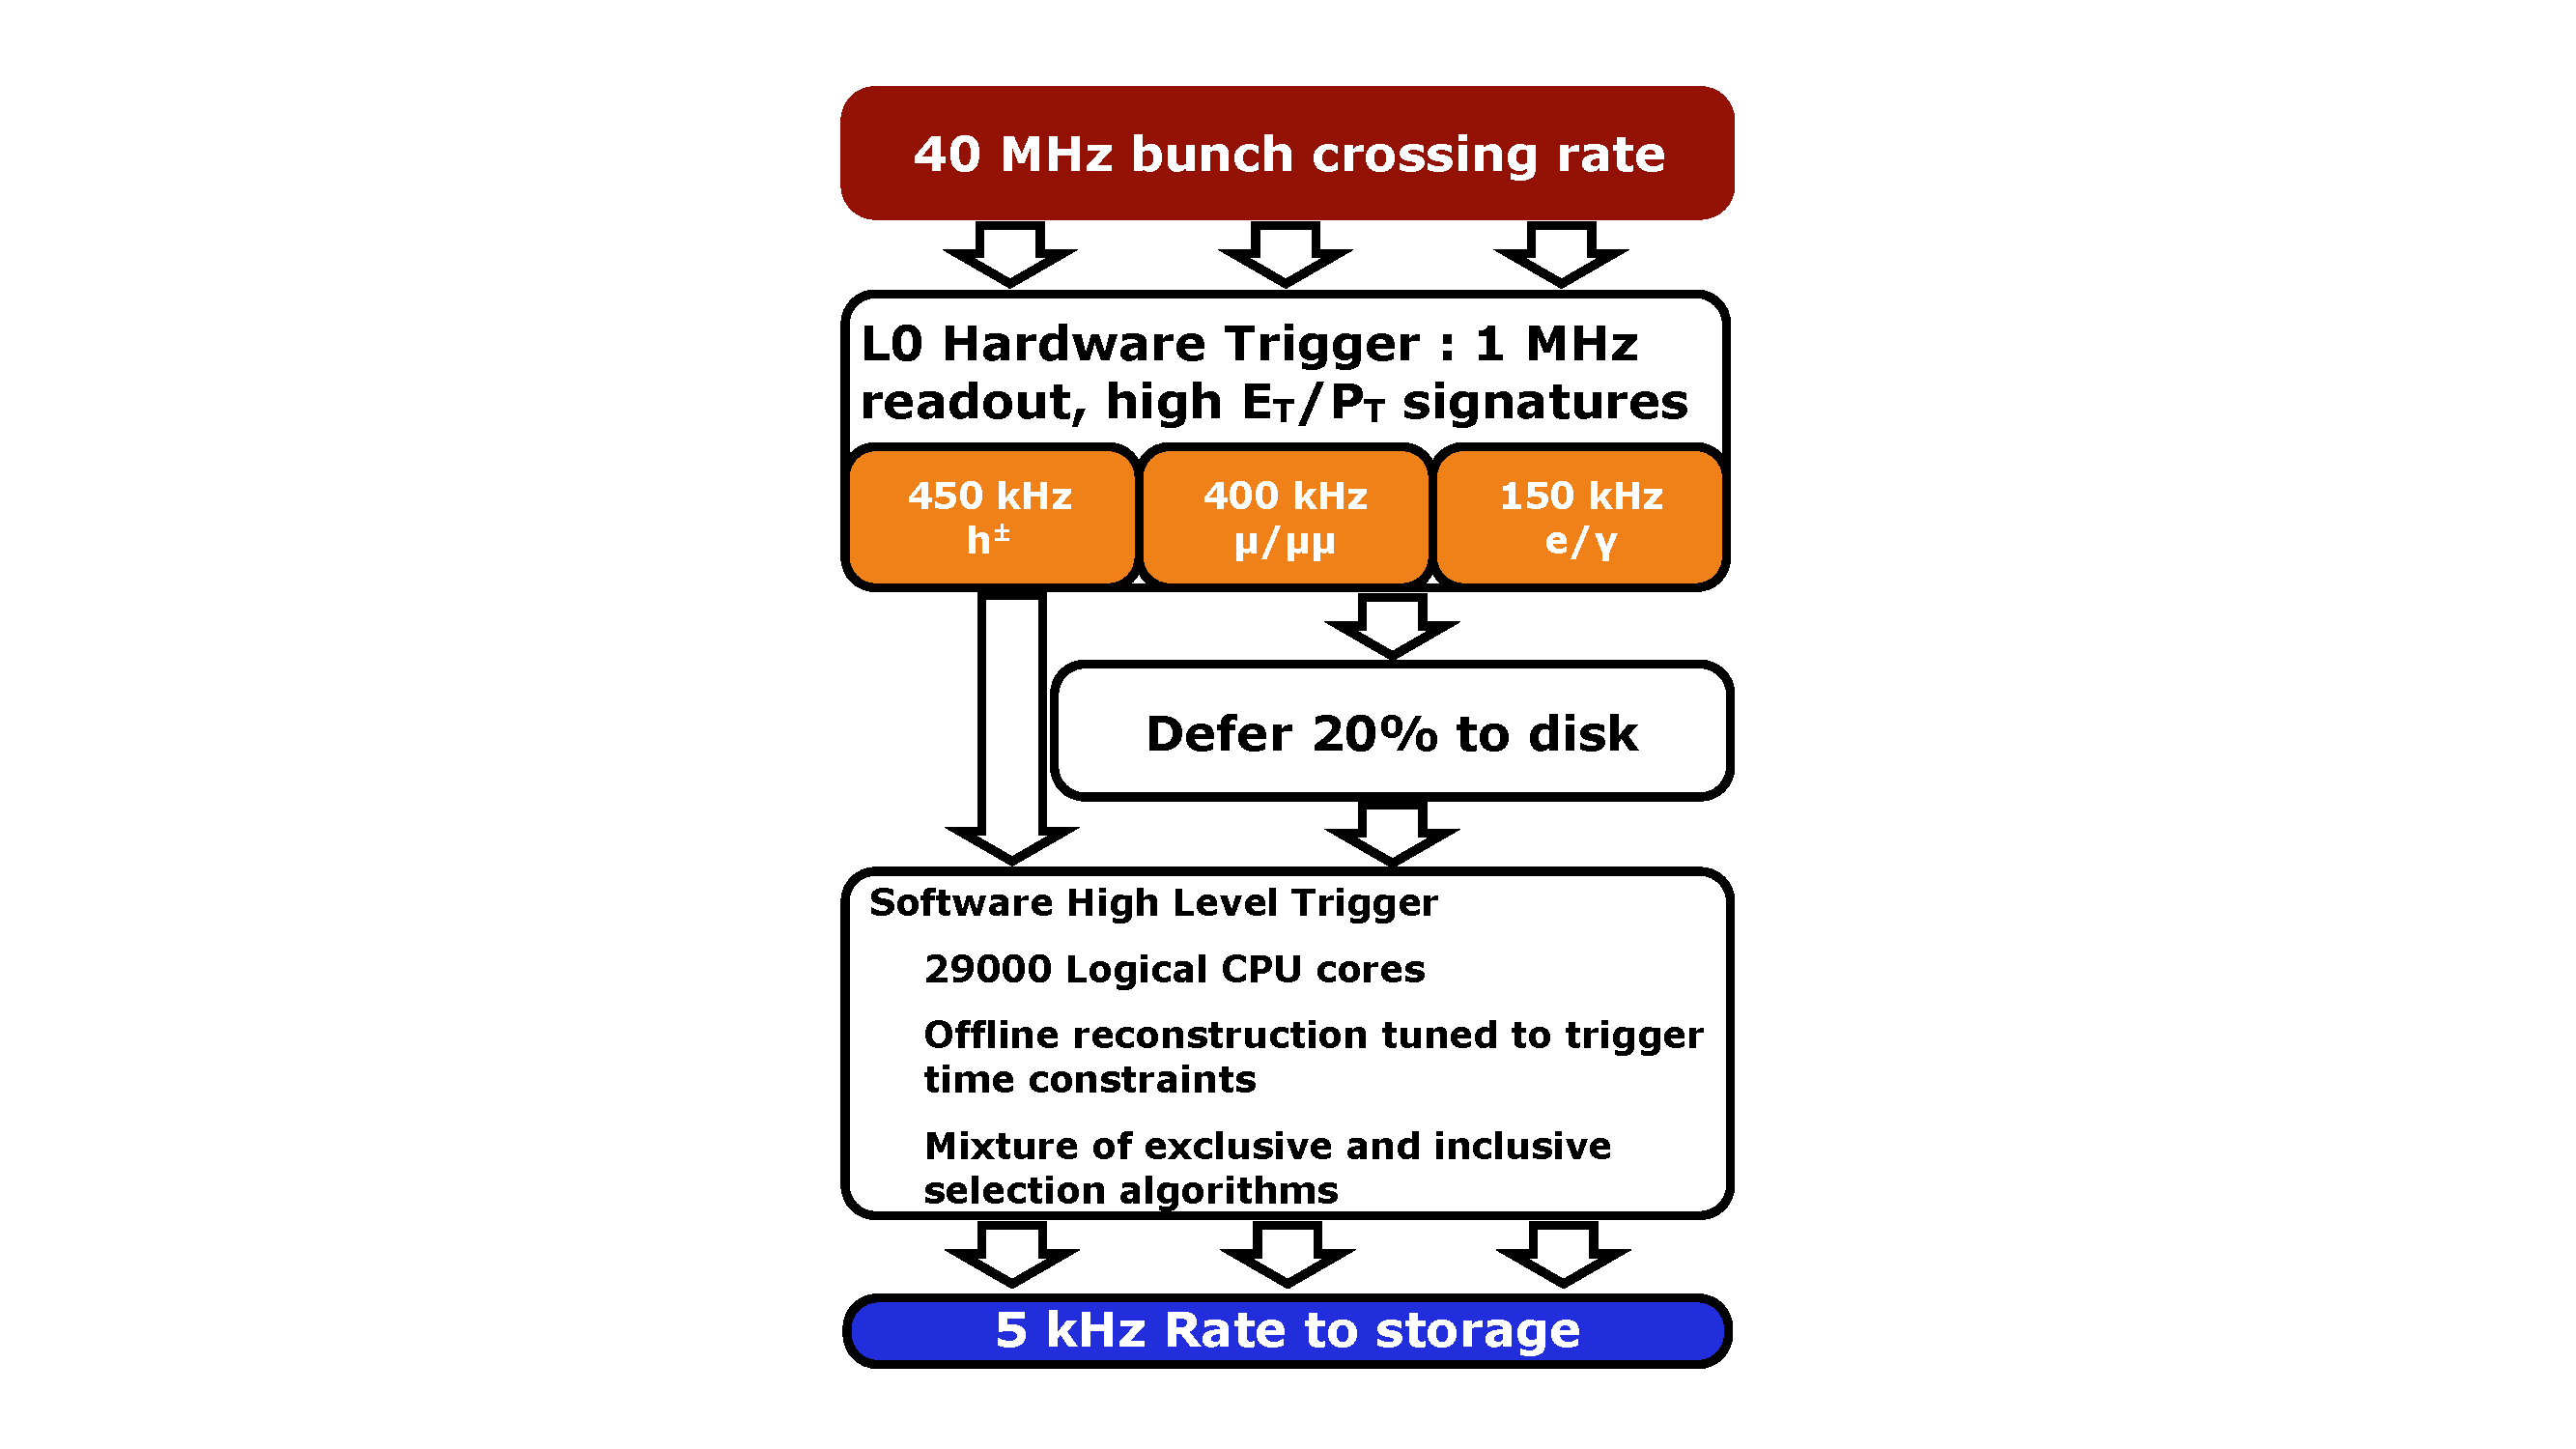
\includegraphics[width=0.45\textwidth, trim={14.5cm 1.4cm 14.5cm 1.4cm}, clip=true]{private/content/the-lhcb-experiment/figs/lhcb_trigger_overview.pdf}
  \caption{
    The \acs{LHCb} \RunOne trigger scheme.
  }
  \label{fig:lhcb_experiment:trigger:overview}
\end{figure}

%%------------------------------------------------------------------------------
\subsection{The \acl*{LZero}}
\label{sec:lhcb_experiment:trigger:lzero}

The \LZero trigger incorporates information from the \VELO pile-up system, the
calorimeters, and the muon system to provide a decision in under
$\SI{4}{\micro\second}$ after the bunch crossing. This reduces the read-out rate
from the \LHC bunch crossing rate of up to $\SI{40}{\mega\hertz}$ to
$\SI{1}{\mega\hertz}$ at which the full detector can be read out. The \LZero
triggers on the highest \ET calorimeter clusters and the two muons with the
highest \pT in the muon system. Additionally global event properties as the
number of primary \protonproton interactions estimated by the \VELO pile-up
system and the number of \SPD hits are used to reject events with large
combinatorics.

%%------------------------------------------------------------------------------
\subsection{The \acl*{HLT}}
\label{sec:lhcb_experiment:trigger:hlt}

To further reduce the data rate the \HLT software trigger handles all events
that pass the \LZero. The \HLT itself is further split into two stages, the
\acs{HLT}1 and the \acs{HLT}2. The first stage performs a partial event
reconstruction using track information from the \VELO, the muon system, and the
main tracking stations to accept events with high \pT tracks. The second \HLT
stage then performs a full event reconstruction on the events passed by the
\acs{HLT}1. Both \HLT stages further reduce the event rate to
$\SIrange[range-units = single, range-phrase = -]{3}{5}{\kilo\hertz}$ before the
data is written to permanent storage.

The \HLT excels in its flexibility and performance, especially regarding the
selection of (di-)muon events. As the \LHC delivers stable physics beams in
about $\SI{30}{\percent}$ of the time, local storage on the computing nodes is
used to \enquote{defer} around $\SI{20}{\percent}$ of the \LZero-passed events
to process them during periods without stable beams \cite{Frank:2014ixa}.

%%%%%%%%%%%%%%%%%%%%%%%%%%%%%%%%%%%%%%%%%%%%%%%%%%%%%%%%%%%%%%%%%%%%%%%%%%%%%%%%
\section{Software stack}
\label{sec:lhcb_experiment:software}

The \LHCb core software framework \Gaudi \cite{set:soft:gaudi} is used for data
processing and supports interfaces to all other software packages. The track
reconstruction is performed by \Brunel \cite{soft:brunel} while \Moore
\cite{soft:moore} runs the \HLTOne and \HLTTwo trigger algorithms. Both packages
differentiate between data and simulation. The generation of simulated events is
managed by the \Gauss \cite{set:soft:gauss} project in consecutive steps: at
first \Pythia \cite{set:soft:pythia} is used as event generator, then the decay
of particles is simulated with \EvtGen \cite{Lange:2001uf} where radiative
corrections are handled by \Photos \cite{set:soft:photos}. The transit of
particle through the detector and the interaction with matter is simulated with
\GeantFour \cite{set:soft:geantfour}. The detector response is finally described
by \Boole \cite{soft:boole} including simulations of electronics noise, detector
cross-talk, and spill-over effects. The \DaVinci \cite{soft:davinci} package
provides an analysis framework to apply selections and---if available---access
\MC informations on reconstructed particle tracks.

%%%%%%%%%%%%%%%%%%%%%%%%%%%%%%%%%%%%%%%%%%%%%%%%%%%%%%%%%%%%%%%%%%%%%%%%%%%%%%%%
\section{Data taking}
\label{sec:lhcb_experiment:data}

Over the \RunOne period from 2010 to 2012 a total integrated luminosity of
$\SI{3.47}{\per\femtobarn}$ was delivered to the \LHCb detector by the \LHC in
\protonproton collisions. The overall data taking efficiency achieved by the
experiment was around $\SI{93}{\percent}$ for the full run period leading to an
recorded integrated luminosity of $\SI{3.22}{\per\femtobarn}$ in \RunOne. The
main sources of efficiency loss can be found in detector dead time, the data
acquisition system, \VELO safety measures, and control of the high voltage
systems. A detailed overview of the data taking history including delivered and
recorded integrated luminosity is depicted in
\cref{fig:lhcb_experiment:data:integrated_lumi}.
%
\begin{figure}[t]
  \centering
  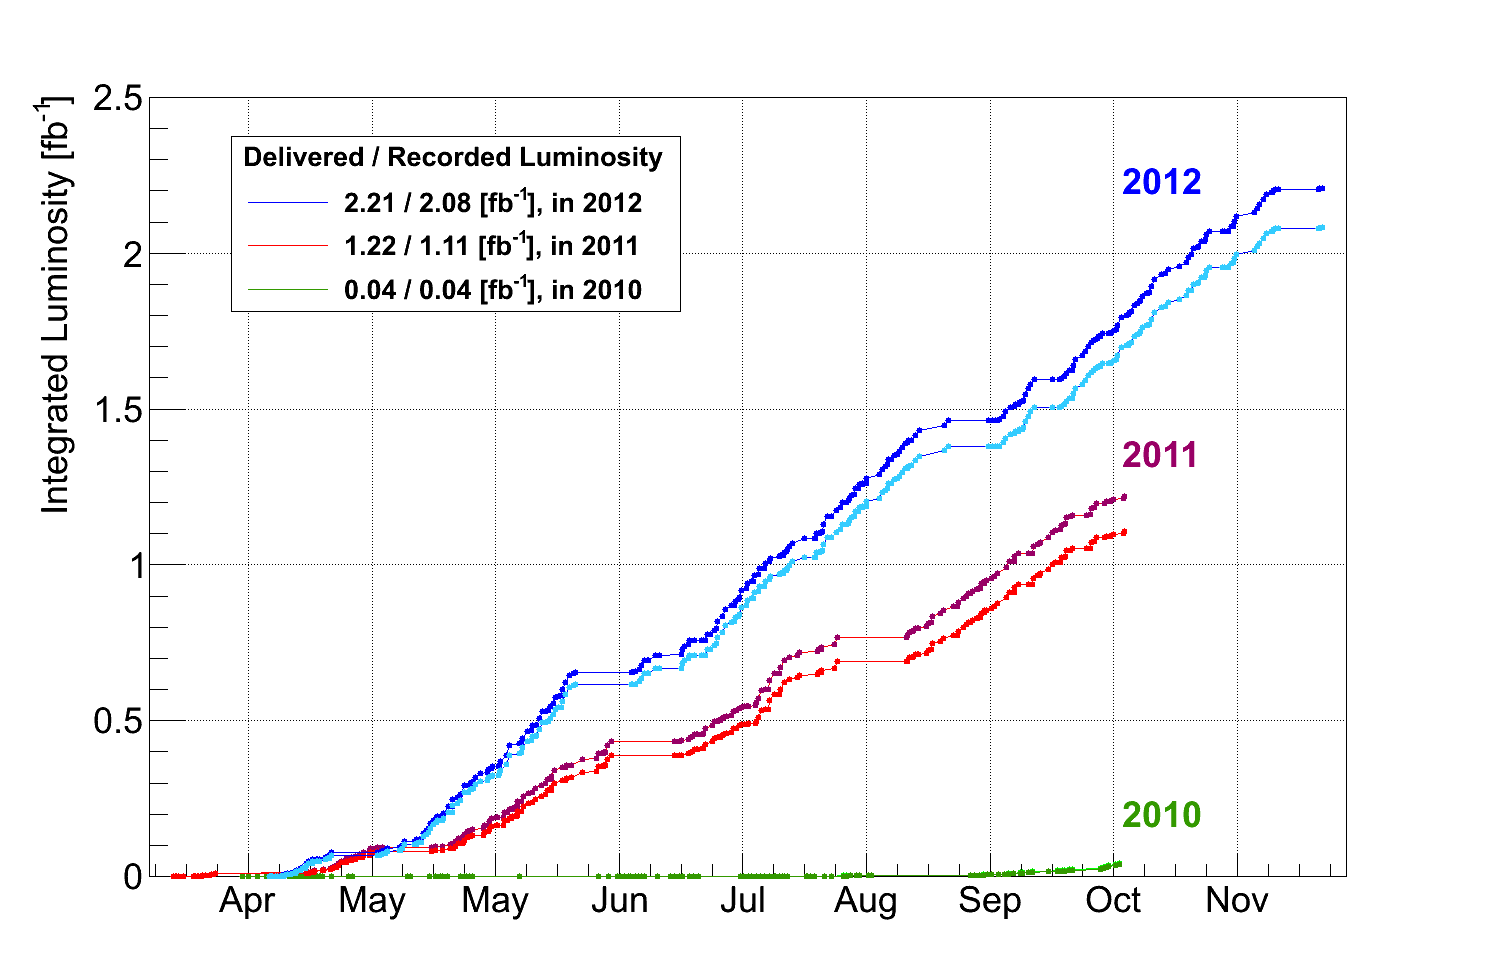
\includegraphics[width=\textwidth]{private/content/the-lhcb-experiment/figs/lhcb_recorded_lumi_runI.png}
  \caption{
    History of delivered and recorded integrated luminosity over the time period
  of \RunOne \cite{lhcb:luminosity}. }
  \label{fig:lhcb_experiment:data:integrated_lumi}
\end{figure}

%%%%%%%%%%%%%%%%%%%%%%%%%%%%%%%%%%%%%%%%%%%%%%%%%%%%%%%%%%%%%%%%%%%%%%%%%%%%%%%%
% \section{\RunTwo and the \acs*{LHCb} upgrade}
% \label{sec:lhcb_experiment:future}

% \missing{\RunTwo and the \acs*{LHCb} upgrade}
% Short description of Run II and Upgrade physics goals, the changes wrt now and what will be possible; a more detailed analysis of the Run II prospects for sin2beta will be given in the conclusions.
